%\documentclass[12pt,a4paper]{report}
\documentclass[12pt,a4paper,oneside,onecolumn,openright]{book}
% set the document language
\usepackage[italian]{babel}
% set the encoding used by your editor here (default is utf8)
\usepackage[utf8]{inputenc}
\usepackage[T1]{fontenc}

% math packages
\usepackage{amsmath}
\usepackage{amssymb}
\usepackage{multicol}
\usepackage{lmodern}
\usepackage{makecell}
\usepackage[table]{xcolor}
\usepackage{colortbl}

% page margins settings
\usepackage[inner=3cm,outer=2.5cm,top=3cm,bottom=2.5cm]{geometry}
%\usepackage{indentfirst}

% other packages
\usepackage{array}
\usepackage{array,multirow,graphicx}
\newcommand{\STAB}[1]{\begin{tabular}{@{}c@{}}#1\end{tabular}}
\usepackage{enumitem}
\usepackage{subfigure}
\usepackage{graphicx}
\usepackage{verbatim}
\usepackage{listings}
\usepackage{url}
\usepackage[hidelinks]{hyperref}
\usepackage[export]{adjustbox}
\usepackage{latexsym}
\usepackage{tabularx}
\usepackage{ragged2e}
\usepackage{mathtools}
\DeclarePairedDelimiter\floor{\lfloor}{\rfloor}
\DeclarePairedDelimiter\ceil{\lceil}{\rceil}
% \usepackage{Mathematics}
% custom colors
\usepackage{color}
\usepackage{wrapfig}
\usepackage{gensymb}
\usepackage{caption}
\usepackage{tikz}
\usepackage{forest}
\usepackage{tikz-qtree}
\usetikzlibrary{positioning, shapes.geometric}
\usetikzlibrary{shapes.geometric, arrows.meta, positioning, fit}
\tikzstyle{block} = [thick, text width=.4cm, minimum height=.5cm, align=center] 


\usetikzlibrary{shadows}
\definecolor{light-gray}{gray}{0.96}
\definecolor{cyan}{RGB}{230,230,255}
\definecolor{dkgreen}{rgb}{0,0.6,0}
\definecolor{gray}{rgb}{0.5,0.5,0.5}
\definecolor{mauve}{rgb}{0.58,0,0.82}
\definecolor{iceberg}{rgb}{0.44, 0.65, 0.82}
% \definecolor{blue}{RGB}{44, 44, 210}

\hypersetup{
colorlinks=true,
linkcolor=black,
% filecolor=blue,
urlcolor=blue,
% pdftitle={Overleaf Example},
}

\urlstyle{same}
\graphicspath{ {./images/} }

\usepackage[many]{tcolorbox}
\newtcolorbox{boxA}{
    % fontupper = \bf,
    boxrule = 1.5pt,
    colframe = black % frame color
}

% environment for bash code
\lstset{ %
  language=bash,                % the language of the code
  basicstyle=\footnotesize,           % the size of the fonts that are used for the code
  numbers=left,                   % where to put the line-numbers
  numberstyle=\footnotesize,          % the size of the fonts that are used for the line-numbers
  stepnumber=1,                   % the step between two line-numbers. If it's 1, each line 
                                  % will be numbered
  numbersep=5pt,                  % how far the line-numbers are from the code
  backgroundcolor=\color{white},      % choose the background color. You must add \usepackage{color}
  showspaces=false,               % show spaces adding particular underscores
  showstringspaces=false,         % underline spaces within strings
  showtabs=false,                 % show tabs within strings adding particular underscores
%  frame=single,                   % adds a frame around the code
  rulecolor=\color{black},        % if not set, the frame-color may be changed on line-breaks within not-black text (e.g. commens (green here))
  tabsize=2,                      % sets default tabsize to 2 spaces
  captionpos=b,                   % sets the caption-position to bottom
  breaklines=true,                % sets automatic line breaking
  breakatwhitespace=false,        % sets if automatic breaks should only happen at whitespace
  title=\lstname,                   % show the filename of files included with \lstinputlisting;
                                  % also try caption instead of title
  numberstyle=\tiny\color{gray},        % line number style
  keywordstyle=\textbf,          % keyword style
  commentstyle=\color{dkgreen},       % comment style
%  stringstyle=\color{mauve},         % string literal style
  escapeinside={\%*}{*)},            % if you want to add a comment within your code
  morekeywords={*,...,insert,-}               % if you want to add more keywords to the setù
}

% environment for python code
\lstset{
	language=Python,
	breaklines=true,
	breakatwhitespace=true ,
	backgroundcolor=\color{light-gray}
}


\newcommand{\grayScale}{0.95} % Can change the gray level here
\definecolor{codeBackground}{rgb}{\grayScale ,\grayScale ,\grayScale}
\definecolor{forestGreen}{rgb}{0.13,0.55,0.13}

\lstset{
    language=C,
    backgroundcolor=\color{codeBackground},
    tabsize=4,
    showstringspaces=false,
    showtabs=false,
    showspaces=false,
    basicstyle=\ttfamily,
    identifierstyle=\ttfamily,
    keywordstyle=\color{blue},
    stringstyle=\color{red},
    commentstyle=\color{gray},
    numberstyle=\color{magenta},
    morecomment=[l][\color{forestGreen}]{\#},
    escapechar={|}, 
}
% appendices package
%\usepackage{appendix}
% set Appendix name used in the toc
%\renewcommand{\appendixtocname}{Appendice}

% interline
\linespread{1.5}
% set numbers for subsections and show them in the toc
\setcounter{tocdepth}{3} 
\setcounter{secnumdepth}{3}

% layout package, style and settings
\usepackage{fancyhdr}
\pagestyle{fancy}

\fancypagestyle{mainmatter}{%		
		\fancyhf{} 
		\fancyhead{}
		\fancyhead[LE,RO]{\thepage}
		\fancyhead[LO]{\footnotesize{\leftmark}}
		\fancyhead[RE]{\footnotesize{\rightmark}}
		\fancyfoot{}
		\addtolength{\headwidth}{\marginparsep}
		\addtolength{\headheight}{2.5pt}
		\renewcommand{\headrulewidth}{0.3pt}
		\renewcommand{\footrulewidth}{0.0pt}
		}
\fancypagestyle{frontmatter}{%
		\fancyhf{} 
		\fancyhead[LE]{\footnotesize{\MakeUppercase{\thepage}}}
		\fancyhead[RO]{\footnotesize{\MakeUppercase{\thepage}}}
		\fancyhead[RE,LO]{}
		\fancyfoot{}
		\addtolength{\headwidth}{\marginparsep}
		\addtolength{\headheight}{2.5pt}
		\renewcommand{\headrulewidth}{0.0pt}
		\renewcommand{\footrulewidth}{0.0pt}
		}
		
		
\usepackage{fancyhdr}
\pagestyle{fancy}
		\fancyhf{} 
		\fancyhead{}
		\fancyhead[LE,RO]{\thepage} 
		\fancyhead[LO]{\footnotesize{\leftmark}}
		\fancyhead[RE]{\footnotesize{\rightmark}}
		\fancyfoot{}
		\addtolength{\headwidth}{\marginparsep}
		\addtolength{\headheight}{2.5pt}
		\renewcommand{\headrulewidth}{0.3pt}
		\renewcommand{\footrulewidth}{0.0pt}

% empty pages have no numbers
\makeatletter
\def\cleardoublepage{\clearpage\if@twoside \ifodd\c@page\else
\hbox{}
  %Potresti voler togliere il commento dalla linea seguente
  %Questa pagina � stata lasciata intenzionalmente vuota.
\thispagestyle{empty}
\newpage
\if@twocolumn\hbox{}\newpage\fi\fi\fi}
\makeatother
%????
%\textwidth=450pt\oddsidemargin=0pt

%\makeatletter 
%  \DeclareRobustCommand*\textsubscript[1]{% 
%    \@textsubscript{\selectfont#1}} 
%  \newcommand{\@textsubscript}[1]{% 
%    {\m@th\ensuremath{_{\mbox{\fontsize\sf@size\z@#1}}}}} 
\makeatother 

\begin{document}
\begin{titlepage}
\begin{center}
{
    \large
    \textbf{Università  degli studi di Modena e Reggio Emilia} \\
   	\textbf{Dipartimento di Ingegneria Enzo Ferrari} \\
    \vspace{\stretch{0.5}}
    \hspace*{0cm} \hrulefill \hspace*{0cm} \\
    \vspace{\stretch{0.5}}    
	  \vspace{\stretch{12}}
  
  
 		\huge{\bf Automotive Connectivity }}\\
		\vspace{3mm}
		
		\vspace{\stretch{6}}
		\end{center}
		
\vspace{40mm}
\par
\noindent
\vspace{20mm}
\begin{center}
\hspace*{0cm} \hrulefill \hspace*{0cm} \\
{\large{\bf 
Anno Accademico 2024/25}}
\end{center}

\end{titlepage}

\pagestyle{frontmatter}
\frontmatter

% PAGINA VUOTA
%\clearpage\null\thispagestyle{empty}\clearpage
\setcounter{tocdepth}{2}
\tableofcontents

\setlength{\parindent}{12pt}
\setlength{\parskip}{1ex plus 0.5ex minus 0.2ex}
\mainmatter
\pagestyle{mainmatter}

\chapter{Introduction}

\section{Structure and Content}
\begin{itemize}

    \item \textbf{Module 1}: 
    \begin{enumerate}
        \item \textbf{\textit{intra-vehicles communications}}: nodes, sensors, ECU
        \item \textbf{\textit{signal busses}}: CAN, LIN, FlexRay, MOST, Ethernet [ T1/T1S]
        \item \textbf{\textit{car domain and OS}}
    \end{enumerate}
    
    \item \textbf{Module 2}:
    \begin{enumerate}
        \item \textbf{\textit{inter-vehicles communications}}: \textit{V2V} and \textit{V2X} (car is a node)
        \item \textbf{\textit{wireless technologies}}: Bluetooth, LoRa, C-V2X, IEE 802.11p (bd)
        \item application, messages, broadcast, GPS
    \end{enumerate}

\end{itemize}
Different \textbf{domain} or \textbf{application} needs different \textit{communications protocols}, is important to understand how each nodes in domain communicate each other (inside the car).

\newpage
\section{Intra-Vehicles}
From the 80's, where the car's control unit are isolated an there was a dedicated wires connect sensors and actuators with less electronic than now, until the reach the greates goal of evolution in the automotive sector: autonomous drive. The complexity of the number of connection from each ECU's to the other, also the number of ECU's for each car, is growing. While the number of signal increase in a liner way, the connection between ECU's is growing with a quadratic complexity $O(n^2)$.

If we examine the evolutions of the ECUs number inside an ``Audi A6'' we can observe that in 1997 it has 5 ECUs and in the 2007 it has 50 ECUs, instead the ``Tesla M3'' in the 2017 has 70 ECUs. The quadratic increase of ECUs number, however has reach a cap for two main reason: the cost and the space inside the car. Traditionally one ECUs is responsible of one task, but nowadays it could be two type of trends:
\begin{enumerate}[nosep]
    \item \textit{distributed of function across ECUs}
    \item \textit{integration of multiple function in one ECU}
\end{enumerate}

\section{Architectures}

\begin{figure}[h]
    \centering
    \begin{minipage}[t]{0.45\textwidth}
        \centering
        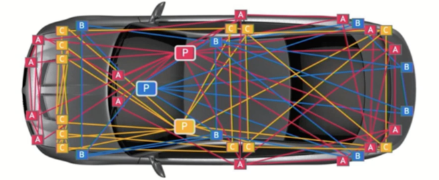
\includegraphics[width=\textwidth]{img/domain_architecture}
        \caption{\textit{Domain Architecture}}
        
        \begin{flushleft}
            \begin{enumerate}[nosep]
                \item central domain controller (\textbf{P}) or high performance computer
                \item ability to handle more complex functions
                \item cost optimization
                \item cable harness is rigid and expensive
            \end{enumerate}
        \end{flushleft}

    \end{minipage}
    \begin{minipage}[t]{0.45\textwidth}
        \centering
        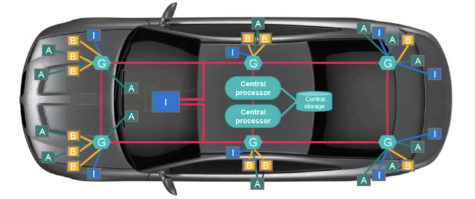
\includegraphics[width=\textwidth]{img/zonal_architecture}
        \caption{\textit{Zonal Architecture}}
        
        \begin{flushleft}
            \begin{enumerate}[nosep]
                \item local ethernet per zone (\textbf{G})
                \item ultra high-speed secured backbone between zone
                \item centralized software
                \item central computer storage
            \end{enumerate}
        \end{flushleft}
        
    \end{minipage}
\end{figure}
\chapter{Intra-Vehicles}

\section{ISO/OSI Layers}
In telecommunication the idea is to divide each steps into layers starting from the application layer to the fisical ones, every layers have different function and it needs different protocols. Each layer can interact with the one that is above or below it and the communication of two layers follow rigid and specifics rules. Nowadays the standard \textit{de iure} is the \textbf{ISO/OSI}, instead the the \textit{de facto} standard is the \textbf{TCP/IP} that relax the rigid guidelines. The \textit{ISO/OSI} has seven layers (bottom to top):
\begin{enumerate}[nosep]
    \item \textbf{physical layer}: specifies the mechanical and electrical properties to transmit bit (in the ``real'' world) and to control time synchronization.
    \item \textbf{data link layer}: checked the transmission of the frame, error checking, frame synchronization and flow control.
    \item \textbf{network layer}: it is used for the transmission of the packets, it is also know as \textit{IP Layer}, in is normally use in ethernet.
    \item \textbf{transport layer}: reliable end to end transport segment, you can manage how the data have to flow. In 99.99 \% of the car domain it doesn't need.
    \item \textbf{session layer}: establish and tear down sessions.
    \item \textbf{presentation layer}: define the syntax and the semantics of information.
    \item \textbf{application layer}: uses data transmitted via physical medium.
\end{enumerate}
In the first module we need only two layers: \textbf{physical layer} and \textbf{data link layer}. We have to study the behaviour of the communication protocols like CANBus, LIN, FlexRay, MOST and Ethernet in this two layers. Starting from the \textbf{transmission medium}, normally the hardware pieces that we use to interact with is:
\begin{itemize}[nosep]
    \item \textbf{transceiver}: is used to ``convert'' analog signal to bits (brain less).
    \item \textbf{controller}: control the communication (brain full).
\end{itemize}
Initially the idea is to focus a little more on \textbf{CANBus}, the \textbf{\textit{Physical Layer}}: is compose by three component: \textbf{Physical Signaling - PLS}, \textbf{Physical Medium Attachment - PMA} and \textbf{Media Dependant Interface - MDI}.
\begin{enumerate}[nosep]
    \item \textbf{physical signaling}: the main purpose is to understand the bit encoding/decoding (if it is \textit{NRZ} or \textit{Manchester}) and to mantein the synchronization all over the network, every transceiver it must have a the same clock source. The synchronization is the most important things both for the bit encoding/decoding and for don't introduce delay in the communication.
    \item \textbf{physical medium attachment}: driver/receiver characteristics based on the communication protocol.
    \item \textbf{media dependant interface}: the connector for access to the physical medium.
\end{enumerate}
\textbf{\textit{Data Link Layer}} is compose by two component: \textbf{Logical Link Control - LLC} and \textbf{Medium Access Control - MAC}.
\begin{enumerate}[nosep]
    \item \textbf{logical link control}: from now on, we start to call \textit{frame} the data that are send/receiver from the physical channel. It is used for \textit{acceptance filtering} that permit to decide if a frame is important for the application above the \textit{controller} and if not discard it. This component include also the \textit{overload notification} and \textit{recovery management} in the case there is an error on the communication they could ask to a re-transmit the data.
    \item \textbf{medium access control}: is purpose is \textbf{error detection} it could check the data encapsulation/decapsulation, frame coding and error detection/signaling/handling.
\end{enumerate}

\section{Network Topology - The Bus System}
\begin{figure}[h]
    \centering
    \begin{minipage}[t]{0.3\textwidth}
        \centering
        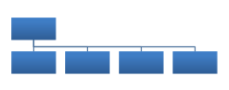
\includegraphics[width=\textwidth]{img/line}
        \caption{\textit{Line Topology}}
        
        \begin{flushleft}
            In the \textbf{Line} topology also know like \textbf{\textit{Bus}} topology each node is connected by interface connectors to a single center cable. It is cheaper than the others and it has lower complexity but it is not very robust.
        \end{flushleft}

    \end{minipage}
    \begin{minipage}[t]{0.3\textwidth}
        \centering
        
\includegraphics[width=\textwidth]{img/star}
        \caption{\textit{Star Topology}}
        
        \begin{flushleft}
            In the \textbf{Star} topology every peripheral nodes is connected to a central node called \textit{hub} or \textit{switch}. It has an higher cost and complexity than the \textit{bus} topology, but it is much more robust (if the \textit{hub} goes down it is a \textit{single point of failure}).
        \end{flushleft}
        
    \end{minipage}
    \begin{minipage}[t]{0.3\textwidth}
        \centering
        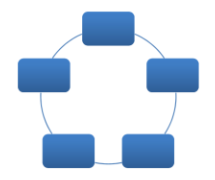
\includegraphics[width=\textwidth]{img/ring}
        \caption{\textit{Ring Topology}}
        
        \begin{flushleft}
            The \textbf{Ring} topology is a \textit{daisy chain} in a closed loop. When a node sends data to another, the data passes through each intermediate node on the ring until reach its destination (it use only one direction). It is not too munch expensive, but has higher complexity (if you want add a new node it could be troublesome).
        \end{flushleft}
        
    \end{minipage}
\end{figure}
In the autonomotive domain it is chosen the \textbf{\textit{Bus Topology}}, why? The first thing is that in the automotive industry it is mandatory to maintain lower the cost. The \textit{busses} are very cheap for the materials, the weight and the volume. In the \textit{bus} topology it is possible to have higher modularity, you can \textit{plug \& play} a node ``when you want'', in that way it is possible to have fully customizability inside the vehicles. The last things is that there is shorter development cycles.
In the autonomotive field there is three main component:
\begin{enumerate}[nosep]
    \item \textbf{\textit{transceiver}}: it is the \textit{physical layer definition} and implement the first layer of the \textit{ISO/OSI} stack.
    \item \textbf{\textit{communication controller}}: it is the communication protocol and implement the first and the second layers of the \textit{ISO/OSI} stack.
    \item \textbf{\textit{ECU}}: also know like \textbf{electronic controller unit} and implement the last layer of the \textit{ISO/OSI} stack, the \textbf{application} layer.
\end{enumerate}
The idea is to made possible to abstract the application layer in order to, if you want, change the first two layers, for example from CANBus to FlexRay, but nothing change at the application layer.

\section{Controller Area Network}
The \textbf{Controller Area Network} also know as \textbf{CAN} is a vehicle bus standard to enable efficient communication. It is originally developed to reduce complexity and cost of electrical wiring. \textbf{\textit{CANBus}} use an \textbf{electrical} medium over wires and a \textbf{broadcast} data transmission. CANBus use the \textbf{\textit{CSMA/CR}} like \textit{multiple access protocol}, it means \textit{carrier sense multiple access collision resolution} protocol, that permit to CANBus to have \textbf{\textit{arbitration}} on the channel access. In this way there is random access to the physical channel, but it is impossible that there is some collision on the communications.
\begin{figure}[h]
    \centering
    \label{img:canbus_1}
    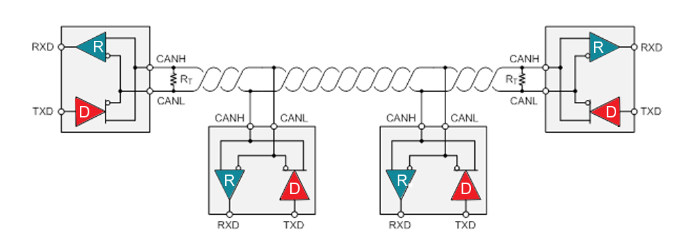
\includegraphics[width=0.75\textwidth]{img/canbus_1}
    \caption{CANBus Network Topology}
\end{figure}

The \textbf{CANBus} network is compose by two wires: \textbf{CAN High} and \textbf{CAN Low}. The data is transmit over the wire using the \textit{potential difference} on each transceiver. Two twisted wires are use because it gives to the protocol \textbf{noise resistance} and \textbf{increase resiliency}, if one brakes, CAN Low \textit{survives}. At the end of the wire in the bus topology there are place two impedance $R_T$ of $120\ohm$. Each CANBus node has three element:
\begin{itemize}[nosep]
    \item \textbf{CAN Transceiver}: is directly connected to the medium access by two pin (one on CANH and the other on CANL). It has the goal to translate the voltage level into bits (during the reception) and send it to the \textit{CAN Controller} and translate bit into voltage level (during the  transmission).
    \item \textbf{CAN Controller}: is connect to the \textit{CAN Transceiver} by two pin (CANTX and CANRX) and is scope is to: message completion, control bus access, transmission and reception of the message, bit timing.
    \item \textbf{Microcontroller}: application software communicating with other ECUs via messages over the bus.
\end{itemize}

\begin{tabular}{ ||p{1cm}|p{2cm}|p{1cm}|p{2cm}|p{2cm}|p{2cm}|p{1cm}|p{1cm}|| } 
    \hline
    \multicolumn{8}{|c|}{ \textbf{CAN Message} } \\ \hline
    1 bit & 29 bit & 1 bit & 6 bit & 0-64 bit & 16 bit & 2 bit & 7 bit\\ \hline
    SOF & CAN-ID & RTR & Control & Data & CRC & ACK & EOF \\ \hline
\end{tabular}

\begin{itemize}[nosep]
    \item \textbf{SOF}: is the \textbf{start of frame} is always set to \textit{dominant \textbf{0}} to tell the other ECUs that a message is coming.
    \item \textbf{CAN-ID}: contains the message identifier - lower value have higher priority.
    \item \textbf{RTR}: is the \textbf{remote transmission request} allow to ECUs to ``request'' message from other ECUs.
    \item \textbf{Control}: informs the lenght of the \textit{Data} in bytes (0 to 8 bytes), two bits are \textit{reserved} for future implementation.
    \item \textbf{Data}: contains the actual data values, which need to be ``scaled'' or converted to be readable an ready for analysis.
    \item \textbf{CRC}: is the \textbf{cyclic rendundancy check} is used to ensure data integrity.
    \item \textbf{ACK}: is the \textbf{acknoledgement} this slot indicates if the CRC is OK all the bits must be \textbf{recessive} (\textit{logical 1}).
    \item \textbf{EOF}: is the \textbf{end of frame} marks the end of CAN message all the bits must be \textbf{recessive} (\textit{logical 1}).
\end{itemize}
The CANBus use a \textit{message passing} technologies, it means, when a message is sent through the wire by an ECUs all the CAN Transceiver reciver the message, but if a application layer of one of another ECUs doesn't need that message it could ignore or if it need it, it could accept that message, using the \textit{CAN-ID} as identifier. In other word the CANBus use the \textbf{receiver-selective} form of addressing. In the CANBus the bit logic is pretty simple, each ECUs reads the wire (through a buffer) and each ECUs \textbf{can} write on the line (through a transistor), in this way the \textbf{basic state} is \textbf{up} ($+5V$ or logical ones) when one or more ECUs want to set signal low turn on transistor conductive (diode), this connect the bus to signal ground in this case the bus level is \textbf{low} ($0V$, or logical zeros) indipendently from other ECUs. The \textbf{0} is named \textbf{dominant level}. It could be see the CANBus wires as \textbf{logical AND} (if an ECUs write zeros the state is \textit{zeros}). \\ \newline
The CANBus is an \textbf{event-driven} bus system, it means that there is no need to wait a scheduled time slot for sending data and there is the possibility of collision over the communication channel. If an ECU $X$ registers an event $e$ it is authorized to access the busses immediately and send data, but if another ECU $Y$ is alredy transmitting data, then $X$ waits. We want to calculate how long it takes a message to be sent, the first thing to do is to calculate the maximum bits number that is allow in a CAN Message: 130 bits. The CANBus can have lots of different bus speed $B \in \{5 k \cdot \frac{bit}{s}, 125 k \cdot \frac{bit}{s}, 250 k \cdot \frac{bit}{s}, 500 k \cdot \frac{bit}{s}, 800 k \cdot \frac{bit}{s}, 1 M \cdot \frac{bit}{s}\}$, let's consider the average $B = 500 k \cdot \frac{bit}{s}$, the resulting time for sending a message is equal to $T_x(time) = \frac{M}{B} = \frac{130 bit}{500 k \cdot \frac{bit}{s}} = 0.25 ms$, but what is happen if two ECUs start the communication on the same time? Let's consider the case where there are three ECUs $X, Y, Z$, $X$ and $Y$ are waiting $Z$ because it is using the medium access, but probably they start to transmit in the same time when the busses is free, in this case we have a \textbf{collision}, the solution is how CANBus implement the \textbf{\textit{CSMA-CR}}, \textbf{carrier sense multiple access - collision resolution}, the two ingredients are how we can see the CAN busses (like a logical AND) and the \textbf{CAN-ID} to the logic prioritizing.
\begin{enumerate}[nosep]
    \item ECU $X$ want to send: it must check if the bus is free (\textit{carrier sense} - \textbf{CR}).
    \item if it is busy the ECU have to wait.
    \item when the bus is free, it could happen that one or more ECUs are ready to transmit, and start the communication together (\textit{multiple access} - \textbf{MA}).
    \item the last incredient is how to avoid the impending damage born from the collsion? (\textit{collision resolution} - \textbf{CR}) $\rightarrow$ \textbf{\textit{bitwise arbitration}}.
\end{enumerate}

All the \textbf{\textit{bitwise arbitration}} is base on the first two field of the CANBus Message: \textbf{SOF} (it is for everyone a \textbf{dominant bit}: \textbf{\textit{0}}) and \textbf{CAN-ID} (it could be 11 bits, in the standard CANBus and 29 bits for the extended ones). We know that in CANBus the ones with the lower \textit{ID} has the greatest priority. Another basic know is that the CANBus network work like a \textit{wired-AND} so if a nodes wrote on the bus a \textbf{\textit{0}} the entire network has logically low value, also if someone else try to wrote a logically high value.

\begin{center}
    \begin{tabular}{ | c | c | c | c | c | c | c | c | c | c | c | c | } \hline
        & \textbf{ID 10} & \textbf{ID 9} & \textbf{ID 8} & \textbf{ID 7} & \textbf{ID 6} & \textbf{ID 5} & \textbf{ID 4} & \textbf{ID 3} & \textbf{ID 2} & \textbf{ID 1} & \textbf{ID 0} \\ \hline
        \textbf{A} & 1 & 1 & 0 & \textcolor{red}{\textbf{0}} & 1 & 0 & 0 & 1 & 1 & 0 & 0 \\ \hline
        \textbf{bus} & 1 & 1 & 0 & \textcolor{red}{\textbf{\textit{0}}} & 1 & 0 & 0 & 1 & 1 & 0 & 0 \\ \hline
        \textbf{B} & 1 & 1 & 0 & \textbf{1} & \multicolumn{7}{ | c }{\makecell{node B loses \textit{arbitration} \\ $\rightarrow$ stop sending and re-start sensing}} \\ 
        \cline{1-5}
    \end{tabular}
\end{center}

\begin{figure}[h]
    \centering
    \begin{minipage}[t]{0.45\textwidth}
        \begin{tabular}{ | c | c | c | } \hline
            \multicolumn{3}{ | c | }{\textbf{wired-and bus logic}} \\ \hline
            \textbf{sender $a$} & \textbf{sender $b$} & \textbf{bus level} \\ \hline
            1 & 1 & 1 \\ \hline
            1 & \textcolor{red}{0} & \textcolor{red}{0} \\ \hline 
            \textcolor{red}{0} & 1 & \textcolor{red}{0} \\ \hline
            \textcolor{red}{0} & \textcolor{red}{0} & \textcolor{red}{0} \\ \hline
        \end{tabular}
        \begin{flushleft}
            We have three knowledge: the default value of the CANBus network is logically high, the bus work as \textit{wired-AND} and the logic \textbf{\textit{0}} si the \textbf{dominant} value, so if the \textit{sender a} or \textit{sender b} send over the bus the \textbf{\textit{0}} value, it win the \textit{arbitration} with the other \textit{sender}.
        \end{flushleft}
    \end{minipage}
    \begin{minipage}[t]{0.45\textwidth}
        \begin{tabular}{ | c | c | c | } \hline
            \multicolumn{3}{ | c | }{\textbf{arbitration logic}} \\ \hline
            \textbf{sender} & \textbf{bus} & \textbf{interpretation} \\ \hline
            0 & 0 & \textbf{next} \\ \hline
            0 & 1 & \textbf{\textit{fault}} \\ \hline
            1 & 0 & \textbf{\textcolor{red}{stop}} \\ \hline 
            1 & 1 & \textbf{next} \\ \hline
        \end{tabular}
        \begin{flushleft}
            We alredy know that CANBus is \textit{carrier sense} if the sender sent over the network a logical \textbf{\textit{1}} but read logical \textbf{\textit{0}} knows that it losts the \textit{arbitration} with another \textit{sender} and have to stops the transmission.
        \end{flushleft}
    \end{minipage}
\end{figure}

\textbf{\textit{Priorities instead of Collision}}: the bus logic and arbitration logic not only prevent collision, it ensure a priority-controlled bus access: smaller ECUs ID, higher priority.
\newpage
\textbf{\textit{CANBus Message Integrity}}: the idea is to use the Data field to generate a CRC to permit the check on the integrity of the message, but wee need some basic knowledge before start: \textit{polynomial division} and \textit{XOR}. 
\begin{boxA}
    \textbf{\textit{Polynomial Reminder Theorem}}: given two polynomials $M(x)$ (the dividend) and $G(x)$ (the divisor), asserts the existence (and the uniqueness) of a quotient $Q(x)$ and a remainder $R(x)$ such that:
    \begin{center}
        \begin{math}
            M(x) = Q(x) \cdot G(x) + R(x)
        \end{math}
    \end{center}
    N.B. the degree of $R(x)$ is stricly lower than the degree of $G(x)$.
\end{boxA}
In the calculation of \textit{CRC} depends on the arithmetic of modulo 2 polynomial. A modulo 2 polynomial is like:
\begin{center}
    $a_n \cdot x^n + a_{n-1} \cdot x^{n-1} + ... + a_2 \cdot x^2 + a_1 \cdot x + a_0$ \\
    $a = \{0, 1\} \quad \forall a \in \{a_0, a_1, ..., a_n\}$
\end{center}
An example of the representation of a binary polynomial is like: $x^3 + x + 1 = 1011$. If exist an $x$ with a certain exponent $e$ like: $x^e$ in the binary representation the position $e$ is fill with a $1$. \\
\begin{center}
    \begin{tabular}{ | c | c | c | } \hline
        $\oplus$ & \textbf{0} & \textbf{1} \\ \hline
        \textbf{0} & 0 & 1 \\ \hline
        \textbf{1} & 1 & 0 \\ \hline
    \end{tabular}
\end{center}
The \textbf{\textit{XOR}} is a digital logic gate that gives a true (logical 1) when the input number is odd, otherwise is false (logical 0). \\ \newline
\textbf{\textit{CRC Encoding}}:
\begin{enumerate}[nosep]
    \item we need to transmit a \textit{n bits} \textbf{message} $M(x)$: $deg(M(x)) = n - 1$.
    \item we have a \textit{m + 1 bits} \textbf{generator} $G(x)$: $deg(G(x)) = m$.
    \begin{itemize}[nosep]
        \item the \textbf{remainder} $R(x)$ of the division $\frac{M(x)}{G(x)}$ will have strictly lower degree respect to $G(x)$ and, in the worst case, the maximum value will be $deg(R(x)) = m - 1$.
        \item $R(x)$ can always expressed with $m$ bits.
    \end{itemize}
    \item add $m$ zeros at the end of $M(x)$: this means to do the following $M(x) \cdot x^m$.
    \item divide the \textbf{new message} $M(x) \cdot x^m$ with the \textbf{generator} $G(x)$ to obtain the \textbf{\textit{reminder}} of \textit{m} bits called \textbf{\textit{CRC}}.
    \item the final message $B(x)$ is equal to $M(x) \cdot x^m + CRC$: this means to add the CRC bits at the end of the message replacing the $m$ zeros padded before.
\end{enumerate}
\textcolor{green}{\textbf{Example}}:
\begin{center}
    $M(x) = 1101011011 \qquad G(x) = 10011 \quad (m = 4)$ \\
    $M(x) \cdot x^m = 11010110110000$
\end{center}
\begin{figure}[h]
    \centering
    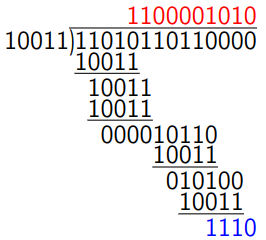
\includegraphics[width=0.3\textwidth]{img/crc_cal}
\end{figure}
The final message $B(x)$ is equal to: $B(x) = \underbrace{1101011011}_\text{M(x)}\underbrace{10011}_\text{R(x)}$ \\ \newline
\textbf{\textit{CRC Decoding}}
\begin{enumerate}[nosep]
    \item the receiver \textbf{acquire} $B(x) = M(x) \cdot x^m + CRC$.
    \item the receiver \textbf{knows} $G(x)$.
    \item the receiver \textbf{divides} the whole message by the generator: $B(x) = \frac{M_x \cdot x^m + CRC}{G(x)}$ 
    \item if the receiver obtain \textbf{no reminder} the transmission was successfully (no errrors detected).
\end{enumerate}
\textbf{\textit{CRC Error Resistance}}: consider an error $E(x)$ occurs on the transmission channel and the receiver $B(x) + E(x)$ instead of simply $B(x)$, when the \textit{CRC logic} can failed? The problem occure when $E(x)$ is multiple of $G(x)$ in this way $\frac{B(x) + E(x)}{G(x)}$ gives no reminder, so the receiver mark $B(x) + E(x)$ as a correct message. To avoid this problem we need to choose in appropriate way the generator $G(x)$, this is the reason why the $G(x)$ it is standard in the \textit{CRC Encoding} (by the protocol). \\ \newline
\textbf{\textit{CRC Design Priciples}}: $G(x)$ is extremely important in a way that $E(x)$ cannot easily be multiple of $G(x)$. For \textbf{detecting single bit of error}:
\begin{itemize}[nosep]
    \item $E(x) = x^i$ for error in i-th bit.
    \item if $G(x)$ has more than 1 term it cannot divide $x^i$.
\end{itemize}
Mathematical theory help us to desing powerful $G(x)$ with fancy characteristics, in CANBus the generator is: $G(x) = x^{15}+ x^{14} + x^{10} + x^8 + x^7 + x^4 + x^3 + 1$. \textbf{sender} and \textbf{receiver} must to agree on the \textbf{generator}. \\ \newline
\textbf{\textit{CANBus bit coding}}: we know that there are two main bit coding algorithm: \textbf{Non return to Zero} (is less noisy) and \textbf{Manchester coding} (carries the clock with him on every single bit). In CANBus is important the clock for the synchronization between nodes, so it could be thinks that \textit{Manchester coding} is the best one to be used. The \textit{Manchester coding} has a big problem: the \textbf{\textit{clock drift problem}}. The \textit{clock drift problem} is \textbf{caused} by natural variations of \textbf{\textit{quartz}} (environment), for the correct working of CANBus the receiver must sample signal at the right time instant. \textit{Clock drift} leads to \textbf{\textit{de-synchronization}} of the clock that comport a bad interpretation of bit sequence. In order to avoid this type of problem, it is necessary to reduce the rising/falling edge of the signal, so it is advise the usage of \textbf{NRZ}.
\begin{boxA}
    \textcolor{red}{\textit{\textbf{Problem}}} \\
    When using \textit{NRZ} coding, sending many identical bits leaves no signal edges that could be used to compensate for the clock drift. \\ \newline
    \textcolor{green}{\textbf{\textit{Solution}}} \\
    Insertion of extra bits after $n$ consecutive identical bits $\rightarrow$ \textbf{\textit{Bit Stuffing}}. In CANBus $n=5$.
\end{boxA}

\newpage
\textbf{\textit{Time Quanta (TQ)}}: is the smallest time slice it could be count. 
\begin{center}
    \centering
    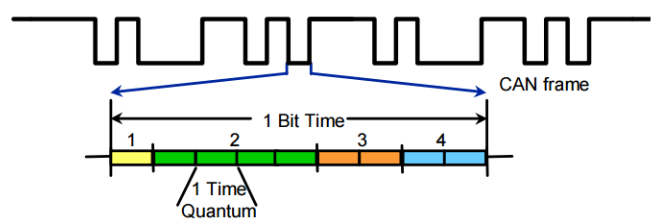
\includegraphics[width=0.75\textwidth]{img/time_quanta}
\end{center}
It is normally divided into four kind of field: \textit{synchronization segment}, \textit{propagation segment}, \textit{phase buffer segment 1} and \textit{phase buffer segment 2}. A \textit{bit} it is compose from 8 to 25 \textbf{time quanta} and it is the smallest discrete timing resolution used by CANBus node. Each \textbf{TQ} is generated by programmable divide of the oscillator. Each segment is composed by an integer number of TQs and segments are non-overlapping. The bitrate is selected by programming the width of the TQ and the number of TQ in the various segments.
\begin{enumerate}[nosep]
    \item \textbf{\textit{synchronization segment}}: it is used to synchronization the various node, only the receiver nodes have to adjust their own clock during the receiver of the payload. The lenght of the segment is always \textbf{1}.
    \item \textbf{\textit{propagation segment}}: if one node transmits to another faraway ones (geographically speaking) how we can synchronize the first \textit{TQ} of the \textit{synchronization segment}? The \textbf{propagation segment} allow the signal propagation across the network and through the nodes. This segment it could be compose from \textit{1 TQ} to \textit{8 TQs} and it is necessary to compensate for signal propagation delays on the bus line and through the electornic interface circuit of the bus nodes.
    \item \textbf{\textit{buffer segment one \& buffer segment two}}: this two segment it could have a programmable lenght between \textit{1 TQ} and \textit{8 TQs}. Between this two segment there is the \textbf{\textit{sample point}}. This point is used from the node to sample the information through the bus channel. This two segment are used to the \textbf{\textit{re-synchronization}}, in some circumstances we need to compensate the oscillator tolerances within the different CAN nodes. 
\end{enumerate}
\begin{boxA}
    \textcolor{red}{\textbf{Jump Width}} \\
    The \textit{jump width} is the amount of \textit{TQs} that we can add (in the \textit{phase buffer segment one}) or remove (in the \textit{phase buffer segment two}) that permit to adjust the lenght during the \textit{re-synch}.
\end{boxA}
Nowadays in many CANBus Modules the \textit{propagation time segment} and \textit{phase buffer segment one} are combined in a new segment named \textbf{\textit{timing segment 1}} (the \textit{phase buffer segment two} is renamed in \textbf{\textit{timing segment 2}}). \\ \newline
\textbf{\textit{Dynamic Sample Position}}: programming the sample point position allow \textbf{flexibility}:
\begin{enumerate}[nosep]
    \item \textbf{\textit{early sample}}: decrease the sensitivity to oscillator tolerances and permit to use lower cost oscillators.
    \item \textbf{\textit{late sampling}}: allow maximum signal propagation time (\textbf{reachability}), maximum bus lenght and poor bus topologies can be handled (more \textit{time quanta} in the \textit{propagation segment}).
\end{enumerate}
\textbf{\textit{CANBus Error}}: there are six possible different error:
\begin{enumerate}[nosep]
    \item \textbf{\textit{Bit-Error}}: write \textit{logical 0} over the bus and sense a \textit{logical 1} (or viceversa). In general if a transmitting ECU detects an \textbf{opposite bit} level on the CANBus we have a \textbf{bit-error}.
    \begin{itemize}[nosep]
        \item ECU writes \textit{logical 0} and reads \textit{logical 1} $\rightarrow$ very bad error.
        \item ECU writes \textit{logical 1} and reads \textit{logical 0} $\rightarrow$ it is ``possible'' when there is the \textbf{bitwise arbitration} or it is expected that the bus state will change to dominant as other nodes acknoledge the message
    \end{itemize}
    \item \textbf{\textit{Stuff Error}}: reminder on the \textit{bit stuffing}: it needs one opposite bit stuffed each 5 consecutive bits, it is used only from the beginning of the frame to the CRC delimiter. From the ACK field to the end is used the \textbf{fixed-form bit fields}. Each node receiving a message that breaks the bit stuffing rules will transmit an \textbf{error frame}.
    \item \textbf{\textit{Format Error}}: if one of the \textit{CRC delimiter field}, \textit{ACK field} or \textit{End Of Frame} have an divergent form, the receiving nodes perform a check to ensure these are correct, if not send a \textbf{error frame}.
    \item \textbf{\textit{CRC Error}}: \textit{CRC delimiter field} is the only weapon to ensure the integrity of the message, it depends on the polynomials division, if the \textit{CRC checks} (the reminder of message plus CRC divided by the Generator) is not $0$ it generates a \textbf{CRC Error}.
    \item \textbf{\textit{General Error}}: the seven \textbf{recessive} bits in the \textit{EOF} are used to inform the CANBus nodes about a general error occured during the transmission. If a receiver node found out an error, it writes six consecutive ``\textbf{zeros}'' forcing an error in the current frame that can be captured from everyone.
    \begin{figure}[h]
        \centering
        \begin{minipage}[t]{0.45\textwidth}
            \centering
            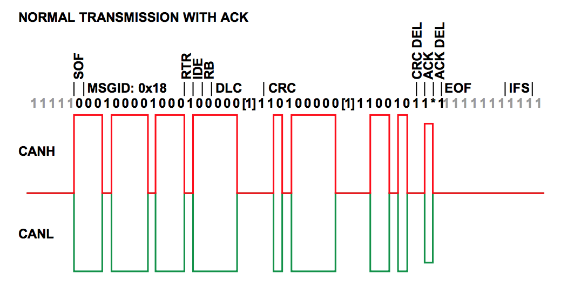
\includegraphics[width=\textwidth]{img/ok_ack}
        \end{minipage}
        \begin{minipage}[t]{0.45\textwidth}
            \centering
            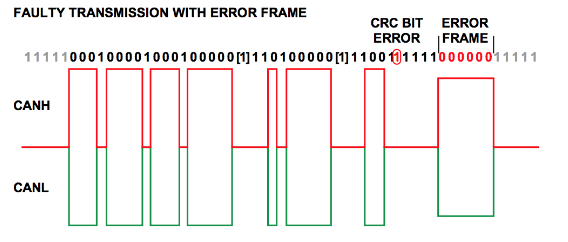
\includegraphics[width=\textwidth]{img/nok_ack}
        \end{minipage}
    \end{figure}
        
    \item \textbf{\textit{ACK Error}}: it happen when no one of the receiver nodes write on the buses an \textbf{dominant} bit in the \textit{ACK field} of the transmitting frame. \\
    \begin{boxA}
        \textbf{\textit{CANBus ACK}} \\
        The transmitting nodes, after the DATA and the CRC, write in the bus a \textit{logical 1} (\textbf{recessive}) and it hopes, in the mean time, that \textbf{at least} one receiver write a \textit{logical 1} (\textbf{dominant}) in the ACK bit, if not the transmitting node (reads on the bus \textit{logical 1}) and will resend the message. \\
        There is two bits for the \textit{ACK field} to absorbe possible delay. We need to allocate space for ``not perfect synchronized receiver'' to push a \textbf{dominant} bit on the bus.
    \end{boxA}
    The \textit{ACK} is triggered by another node so the voltage value could be slightly different. These technologies have some implication on the CANBus protocol, like:
    \begin{itemize}[nosep]
        \item also the recevier node/s can (have to) transmit during specific frame slot (the \textit{ACK field} or \textit{EOF}).
        \item all the receiver must check the \textit{CRC} very quickly in order to know if the message have pass the integrity checks.
        \item a CANBus network \textbf{\textit{must have at least two nodes to work}}, because with only one node no one can acknoledge a message.
    \end{itemize}
\end{enumerate}
For the calculous of the time in the circuit (in the CANBus controller) it is normally used \textbf{\textit{time crystal}}, the smallest \textit{ICs} possible is the $8MHz$ \textit{time crystal}. If we consider each clock cycle for the smallest unit in CANBus (\textit{time quanta}) for each bit we have at least \textit{8 TQs} (up to \textit{25 TQs}). \\
If we minimize the size of the of a single bit we have to consider \textit{8 TQs}. $\frac{8MHz}{8 TQs} = 1MHz$ we can obtain the maximum bitrate for the CANBus. \\ \newline
\textbf{CANBus Recap}:
\begin{enumerate}[nosep]
    \item \textbf{\textit{low cost}}: the price is \textbf{always} a costraint, with it's two wires has a good price-performance tradeoff. This enables the use of CANBus outside the autonomotive domain.
    \item \textbf{\textit{reliability}}: CANBus has sophisticated error detection and handling mechanisms. If failed the integrity checks of the frame it could repeat the sending of the same data and every nodes are informed about the error. CANBus has high immunity to EMI.
    \item \textbf{\textit{latency}}: CANBus means real-time (soft) because there is low latency between transmission and request and actual start of transmission. CANBus has inherent arbitration on message priority due to the bitwise arbitration logic.
    \item \textbf{\textit{flexibility \& speed}}: CANBus nodes are ``plug \& play'' and there are not limited number of nodes into a network.
    \item \textbf{\textit{multi master operation}}: (ECU peers) each nodes is able to access to the bus, if there is a fulty nodes the bus communication is not disturbed and they switch-off from the communication.
    \item \textbf{\textit{broadcast capabilities}}: message can be sento to single/multiple nodes and every node simultaneously receive common data. 
    \item \textbf{\textit{Standardize}}: \textit{ISO-DIS 11898} (high speed), \textit{ISO-DIS 115192-2} low speed.
\end{enumerate}

\newpage
\section{Controller Area Network Flexible Data-Rate}
The \textbf{\textit{CAN-FD}} is the evolution of the \textit{CANBus}. The mainly disadvantages of CANBus are: $1MHz$ in some circumstances are not enough and only \textit{8 bytes} of payload are often restrictive. To be compliant to standard CANBus the \textit{arbitration phase} (before the data) and \textit{ACK phase} (after the data) must be mantein to the same frequency. \\
CAN-FD data frames can be transmitted with two different bit-rates, in the \textit{arbitration phase} and in the \textit{ACK phase} the bitrate depends on the network topology and it is limited to $1MHz$, instead in the \textit{data phase} the bitrate is limited by the \textit{transceiver characteristics}:
\begin{itemize}[nosep]
    \item support a bitrate higher than $1MHz$.
    \item support a payload larger than \textit{8 bytes}.
\end{itemize}
The increase of the frame speed is possible by shortening the bit time. We define the \textbf{\textit{Bit Rate Shift - BRS}} is the bit in the \textit{control field} used to inform \textbf{ALL} the nodes that sender will transmit faster in the \textit{data transmission phase} and the \textbf{\textit{Extended Data Lenght - EDL}}. The implication of this change are:
\begin{itemize}[nosep]
    \item \textbf{larger payload}: it needs more \textit{CRC bits} to maintain the robustness of CANBus, to have more \textit{CRC bits} it needs a \textbf{larger generator}.
    \item \textbf{shorter bit-time}: new bit-time logic in the state machine, a \textit{factor} is introduce between the bit time during arbitration phase and the bit-time during the transmission. The tipical factor is 8 $\rightarrow$ considerering the fastest rate of CANBus \textit{arbitration phase} and the longer header and CRC, the final result is more or less $6MHz$.
\end{itemize}
\begin{figure}[h]
    \centering
    \label{img:canfd}
    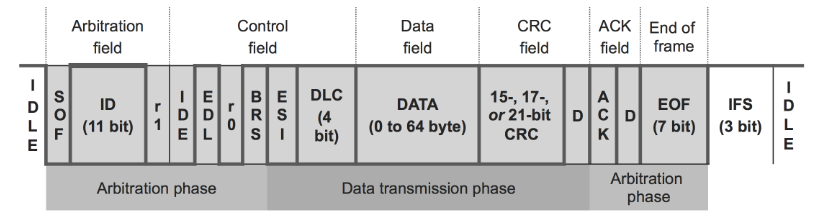
\includegraphics[width=0.75\textwidth]{img/can_fd}
\end{figure}
To summarize the \textbf{CAN-FD} could reach in the \textit{data transmission phase} the speed transmission of $6MHz$ and the possibility of sending a payload large up to \textbf{64 bytes}

\newpage
\section{Local Interface Network}
\begin{center}
    \label{fig:can_lin}
    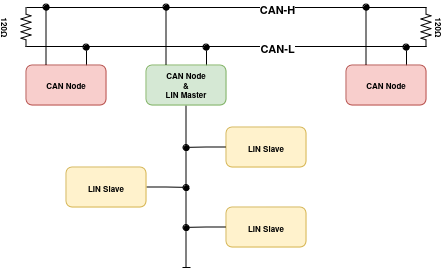
\includegraphics[width=0.5\textwidth]{img/can_lin}
\end{center}
The \textbf{\textit{LIN}} is a message oriented communication protocol that is design and developed to create something cheaper than low speed CANBus, this purpose it was reach partaway. Like the CANBus, LIN, works on the first two layers of the ISO/OSI stack (physical and data link layers), but it uses a \textbf{master-slave} concept. Using this architecture, the LIN busses, can have only a quartz on the master that manage the synchronization on all the LIN network, to achieve without waste space on the vehicle, the master of the LIN mesh is part of the CANBus network. This is the reason why the LIN is also know like a \textbf{\textit{sub bus}} of CANBus (Fig. \ref{fig:can_lin}). As result on the communication we can say that LIN network is self-synchronize, but for this reason it needs to have lax timing constraints because only one node (the \textbf{master}) can schedule the order of the transmission. In addition to this, LIN busses, has other difference between CANBus:
\begin{itemize}[nosep]
    \item LIN is a \textbf{bidirectional one-wire line} and it can reach the frequency up to $20kHz$ (CANBus can reach $1MHz$).
    \item The \textbf{voltage} for the analog transmission over the channel is 40V, instead the CANBus is only up to 5V.
    \item \textbf{Bit Transmission} is \textit{UART} like:
    \begin{center}
        \begin{tabular}{ | c | c | c | } \hline
            \multicolumn{3}{|c|}{\textbf{bit transmission}} \\ \hline
            1 bit & 8 bits & 1 bit \\ \hline
            \textbf{start bit} & \textbf{data bits} & \textbf{stop bit} \\ \hline
        \end{tabular}
    \end{center}
\end{itemize}
In LIN protocol there is a rudimental error detection on the frame, it is a sum of all the payload bytes modulo 256 (in this way it can be stored into a single byte), but also on the channel, if a sender while monitoring the bus, read an unexpected state abort the communication without correction. The \textbf{schedule} of the network is hardcoded on the \textbf{master's firmware} (static), the scheduler determines which node have to transmit in that specific slice of time. This consent to have a channel that is \textbf{mostly deterministic}, permit to the slave to not know how it is schedule the transmission and allow to the master to \textit{change the order of transmission runtime}. \\ \newline
\textbf{\textit{LIN Message}}: is divide into two component: \textit{Message Header} and \textit{Message Response}. The first one is sent over the channel by the \textbf{maaster node} and is like a request for a specific slave, instead it is possible to see the second one like the slave response.
\begin{center}
    \begin{tabular}{ | p{2cm} | p{1cm} | p{2cm} | p{5cm} | p{2cm} | } \hline
        \multicolumn{3}{|c|}{\textbf{Message Header}} & \multicolumn{2}{|c|}{\textbf{Message Response}} \\ \hline
        \textit{Break} & \textit{Sync} & \textit{Identifier} & \textit{Data} & \textit{Checksum} \\ \hline
        14 bits & 8 bits & 8 bits & 0 to 64 bits & 8 bits \\ \hline
    \end{tabular}
\end{center}
Description for each field:
\begin{enumerate}[nosep]
    \item \textbf{\textit{Break}}: is composed by two kinds of fields: \textbf{13 low bits} (\textit{dominant}) and \textbf{1 high bit} (\textit{recessive}) that is used to delimiter of the field.
    \item \textbf{\textit{Sync}}: is used to \textit{synchronize} the bit timing of the slave, it is always \textbf{0x55} (01010101) in this way follow the profile of the clock.
    \item \textbf{\textit{ID}}: is used to individuate the right slave, different from the CANBus, in this identifier there are parity bit, to have a check on the integrity of the ID, because in this case is very important for the correct master-slave communication (\textbf{protected field}). ID is divide in two segment:
    \begin{itemize}[nosep]
        \item from \textbf{LIN 2.0} the first \textbf{2 MSB bits} define the lenght of the payload that could be 2, 4 or 8 bytes, previous version of LIN used static 8 bytes data lenght.
        \item \textbf{4[6] bits} for the ``real'' ID.
        \item \textbf{2 parity bits}:
        \begin{center}
            $p_0 = id_0 \oplus id_1 \oplus id_2 \oplus id_4$ \\
            $p_1 = id_1 \oplus id_3 \oplus id_4 \oplus id_5$
        \end{center}
    \end{itemize}
    \item \textbf{\textit{Data}}: contain the payload, and it was send by the slave selected by the master with the lenght settled in the identifier.
    \item \textbf{\textit{Checksum}}: is this case, like said before, the checksum is the sum of all the payload bytes modulo 256, in that way it can be stored into a single byte.
    \begin{center}
        \begin{tabular}{ | c |  c |  c |  c |  c |  c |  c |  c |  c | } \hline
            & $d_7$ & $d_6$ & $d_5$ & $d_4$ & $d_3$ & $d_2$ & $d_1$ & $d_0$ \\ \hline
            \textbf{carry} & & \textcolor{red}{\textit{1}} & \textcolor{red}{\textit{1}} & \textcolor{red}{\textit{1}} & & \textcolor{red}{\textit{1}} & & \\ \hline
            \textbf{first byte} & 0 & 0 & 0 & 1 & 0 & 1 & 1 & 0 \\ \hline
            \textbf{second byte} & 0 & 0 & 0 & 1 & 0 & 1 & 1 & 1 \\ \hline
            \textbf{third byte} & 0 & 0 & 0 & 1 & 0 & 1 & 1 & 0 \\ \hline
            \textbf{forth byte} & 0 & 0 & 0 & 1 & 0 & 0 & 0 & 0 \\ \hline
            \textbf{fifth byte} & 0 & 0 & 0 & 1 & 0 & 0 & 0 & 0 \\ \hline
            \textbf{\textit{checksum}} & \textbf{0} & \textbf{1} & \textbf{1} & \textbf{0} & \textbf{0} & \textbf{0} & \textbf{1} & \textbf{1} \\ \hline
        \end{tabular}
    \end{center}
\end{enumerate}
LIN nodes are typically bundled in clusters each with a master that interfaces with the backbone CANBus. We have introduce the general message/frame format, but in LIN protocol there are six kinds of different messages (encoded in the ID field):
\begin{enumerate}[nosep]
    \item \textbf{\textit{Unconditional Frames}}: is defined by the ID \textbf{\textit{0x00 - 0x3B}} and is the default type of frame, where the master send a header over the channel and the request slave reply.
    \item \textbf{\textit{Event Trigger Frames}}: is defined by the ID \textbf{\textit{0x00 - 0x3B}}, the master polls multiple slaves, the slave who have updated data response, if there are collision, the communication end and the master switch to \textit{unconditional frame}.
    \item \textbf{\textit{Sporadic Frames}} is defined by the ID \textbf{\textit{0x00 - 0x3B}} in this type of message the master acts like a slave and reply to his own requests.
    \item \textbf{\textit{Diagnostic Frames}} is defined by the ID \textbf{\textit{0x3C - 0x3D}} with this frame the communication becomes request-response, the \textbf{\textit{0x3C}} is the ID where the master make the request, instead the \textbf{\textit{0x3D}} is the ID where the slave reply.
    \item \textbf{\textit{User Defined Frames}} is define by the ID \textbf{\textit{0x3E}} is a user-defined frame and it can contain any types of information.
    \item \textbf{\textit{Reserved Frames}}: ID \textbf{\textit{0x3F}}
\end{enumerate}
There is a reason why the \textbf{data lenght} of CANBus and LIN are equal. Since LIN is also called CANBus sub system, for compatibility reason the payload is equal. Message of CANBus can be sent over LIN too and viceversa.
\chapter{Inter-Vehicles}

\section{Global Positioning System}
The \textbf{\textit{GPS}} in origin named \textbf{NAVigation Satellite Timing and Ranging Global Positioning System} (\textbf{NAVSTAR GPS}) is one of the space-based \textit{global navigation satellite system} (\textbf{GNSS}) that provides \textbf{geolocation} and \textbf{time information} anywhere on the Earth, using the signal of at least four satellite. The geolocation information gives an \textbf{XYZ} coordinates.

\subsection{Actors}
\textbf{GPS} is based on three elements: \textbf{space segment} (the satellite), \textbf{control segment} (ground station) and \textbf{user segment} (end-user equipments):
\begin{enumerate}[nosep]
    \item \textbf{space segment}: have the main goal to broadcast navigation message constantly.
    \item \textbf{control segment}: ground antennas that \textit{track}, \textit{collect} and \textit{correct} all the \textbf{sat orbits} (normally they are very precise and known a priory). They both recive/transmit data from/to satellites.
    \item \textbf{user segment}: cheap devices used to collect GPS signal and know the position (it has the maximum error approximately of 1 meter).
\end{enumerate}

\subsection{NAV Msg}
The information \textbf{broadcasted} by the satellite is called \textbf{\textit{Navigation Message}} (\textbf{NAV}). The nav msg is composed by:
\begin{figure}[h]
    \centering
    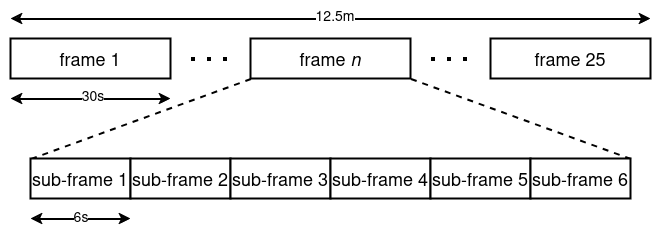
\includegraphics[width=0.75\textwidth]{img/gps_frame}
\end{figure}
\begin{itemize}[nosep]
    \item \textbf{25 frames} (or \textbf{pages}) that takes 12.5 minutes to be transmitted.
    \item each frame takes 30 seconds to be transmitted and it is formed by \textbf{6 sub-frame}.
    \begin{enumerate}[nosep]
        \item the first sub-frame contains the \textbf{satellite clock information}.
        \item the second and the third give the information about the \textbf{satellite ephemeris} (\textbf{orbit}).
        \item the forth and thr fifth are different and are complete only receiving all the 25 frames of the NAV msg, they have the \textbf{Almanac \& constellation status}.
    \end{enumerate}
    \item each sub-frame needs 6 seconds to be transmitted, and it is composed by \textbf{10 words}.
    \item each word consist of \textbf{30 bits} and it takes 0.6 second to be transmitted.
\end{itemize}

\newpage
\subsection{Bit Coding}
GPS use the \textbf{Bi-Phase Shift Key} (\textbf{BPSK}) modulation technique. In BPSK the carrier signal is modified by altering its phase by 180 degree, for each symbol. A phase shift of 180 degrees denotes a binary 0 while no phase shift represents a binary 1. The advantages to use this type of mudaltion technique is:
\begin{enumerate}[nosep]
    \item rendundancy
    \item jamming resistance
    \item measure \& remove the ionospheric delay
    \item requires a dual frequency receiver (with a single one it is possible to survive but less accuracy) one at $1575.42MHz$ and the other one at $1227.60MHz$.
\end{enumerate}
\begin{figure}[h]
    \centering
    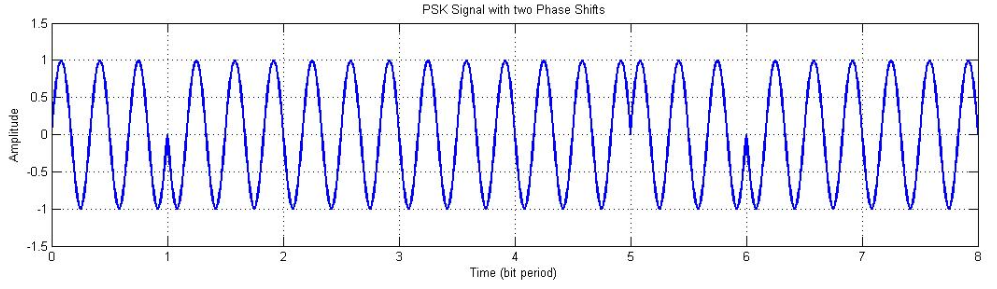
\includegraphics[width=\textwidth]{img/bspk_wave}
\end{figure}
\begin{figure}[h]
    \centering
    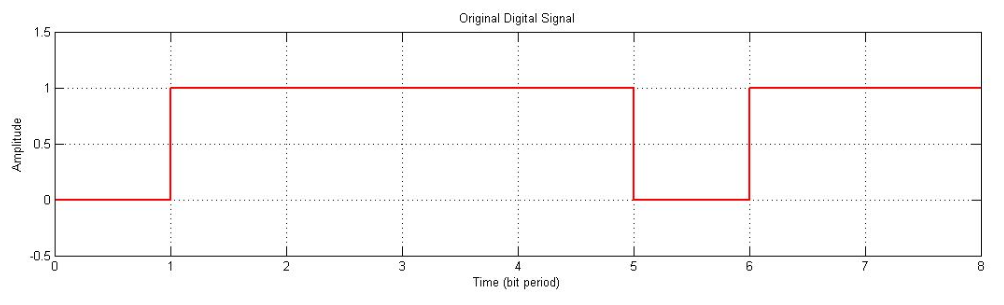
\includegraphics[width=\textwidth]{img/bspk_signal}
\end{figure}

\newpage
\subsection{Working Principle}
Let's distinguish the study of the working principle in two hypotheses: \textbf{theoretical}: receiver clock is perfectly synchronize with the satellite clock (\textit{absolute clock}); and \textbf{reality}: receiver clock is cheap, non-atomic and not perfectly synchronize with the satellite clock.

\begin{figure}[h]
    \centering 
    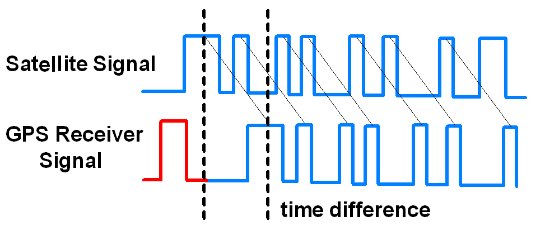
\includegraphics[width=0.45\textwidth]{img/hp_theory}
    \caption{Satellite-Receiver clock synch}
\end{figure}
In the first hypothesis, we know: \textbf{satellite position} (written in the NAV), \textbf{satellite clock} (written in the NAV) and the \textbf{speed of light} $c$. So it is possible to obtain:
\begin{enumerate}[nosep]
    \item \textbf{signal travel time}: $\Delta t = clock_{recv} - clock_{NAV}$
    \item \textbf{distance satellite-receiver}: $d = c \cdot \Delta t$
\end{enumerate}
The problem is, if there is at least $1ms$ of de-sync between the satellite and the receiver, then will have at least an error of 200 miles.
Solution: \textbf{\textit{Trilateration}}.

\begin{figure}[h]
    \centering
    \begin{minipage}[t]{0.3\textwidth}
        \centering
        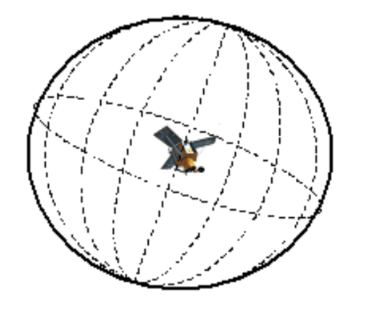
\includegraphics[width=0.7\textwidth]{img/gps_one}

        \begin{flushleft}
            if it is knows \textbf{one} $sat_i$ and the distance $d_i$ we can be in any point of the spherical surface of radius $d_i$ centered in $sat_i$.
        \end{flushleft}
    \end{minipage}
    \begin{minipage}[t]{0.3\textwidth}
        \centering
        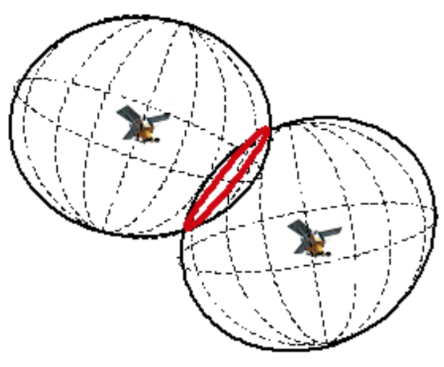
\includegraphics[width=0.7\textwidth]{img/gps_two}

        \begin{flushleft}
            if the sat known are \textbf{two} $sat_i$ and $sat_j$ both the position and the distance $d_i$, $d_j$ we can be in any point of the border given by the intersection of the two sphere's surface.
        \end{flushleft}
    \end{minipage}
    \begin{minipage}[t]{0.3\textwidth}
        \centering
        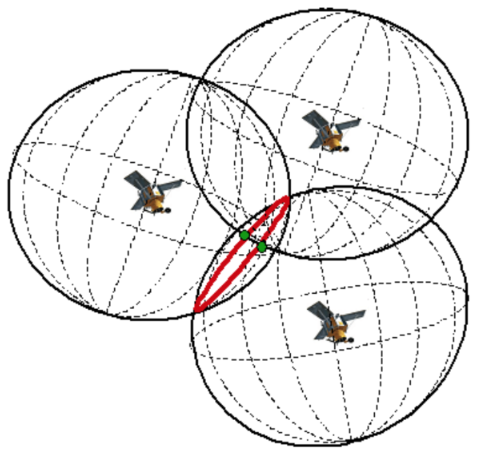
\includegraphics[width=0.7\textwidth]{img/gps_three}

        \begin{flushleft}
            adding the \textbf{third} sat, we have \textbf{three} sphere, that ends the intersection with two available points. One is on the Earth surface (us) the other is in the open space (discard).
        \end{flushleft}
    \end{minipage}
\end{figure}
In the \textbf{reality} the satellite and the receiver do not have the clock synchronize, so it is important to introduce a factor named \textit{clock error} $\Delta e$:
\begin{center}
    $d_i = \sqrt{(x_i - x_u)^2 + (y_i - y_u)^2 + (z_i - z_u)^2} + c \cdot \Delta e$
\end{center}
where:
\begin{itemize}[nosep]
    \item $x_i$, $y_i$ and $z_i$ are the sat position, \textbf{know} (NAV).
    \item $c$ is the speed of light, \textbf{know}.
    \item $x_u$, $y_u$ and $z_u$ are the position of the receiver, \textbf{unknown}.
    \item $\Delta e$ is the clock error, \textbf{unknown}.
\end{itemize}
If we consider four satellites $sat_i$, $sat_j$, $sat_k$ and $sat_p$ we end with four equations and four unknown items: $x_u$, $y_u$, $z_u$ and $\Delta e$.
\begin{center}
    \begin{math}
        \begin{cases}
            d_i = \sqrt{(x_i - x_u)^2 + (y_i - y_u)^2 + (z_i - z_u)^2} + c \cdot \Delta e \\
            d_j = \sqrt{(x_j - x_u)^2 + (y_j - y_u)^2 + (z_j - z_u)^2} + c \cdot \Delta e \\
            d_k = \sqrt{(x_k - x_u)^2 + (y_k - y_u)^2 + (z_k - z_u)^2} + c \cdot \Delta e \\
            d_p = \sqrt{(x_p - x_u)^2 + (y_p - y_u)^2 + (z_p - z_u)^2} + c \cdot \Delta e
        \end{cases}
    \end{math}
\end{center}
$\Delta e$ is equal for all satellite, because all of them are perfectly synchronize, so the \textit{clock error} is the same for each tuples (sat, recv). If recv and sat are perfectly synchronize (\textbf{time} given), with just 3 sat is possible to calculate your position. If you know where you are (\textbf{space} given), with just one sat is possible to have the clock sync, but if you do \textbf{not know} both \textbf{space} and \textbf{time} you need at least four sat to solve the equation.

\subsection{GPS limitation}
\begin{itemize}[nosep]
    \item it require a lot of power to work properly.
    \item GPS signal do not pass solid structure.
    \item affected by large buildings, unreliable in dense urban area.
    \item GPS accuracy is function of the signal reception, larger the antenna, better the signal. $miniaturization \quad \frac{1}{\alpha} \quad accuracy$
\end{itemize}

\newpage
\section{Bluetooth}
\textbf{\textit{Bluetooth}} is short-range wireless technology and it was introduce for the first time in 1994 to replace serial \textit{RS-232} wired cables. Typically used for \textbf{point-to-point} technologies. It has a coverage of 10m and creates a network named \textbf{Personal Area Network} (\textbf{PAN}), the frequency range is between $2.4GHz$ and $2.485GHz$ with few $Mbps$ of bandwidth. It is standardize in the \textit{IEEE 802.15.1} like packet-base protocol.

\begin{figure}[h]
    \centering
    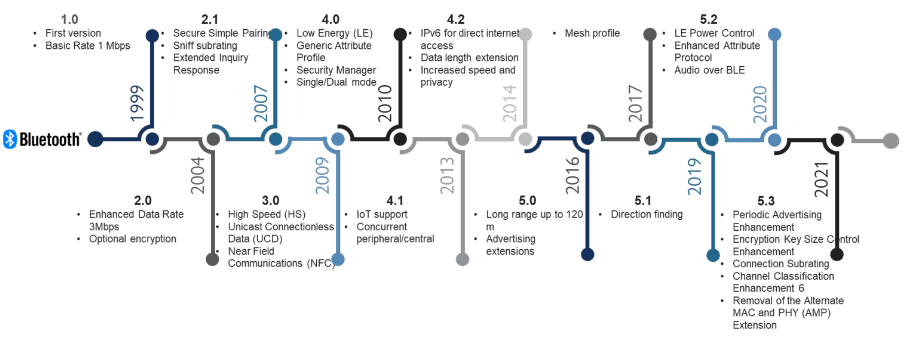
\includegraphics[width=\textwidth]{img/bluetooth_timeline}
    \caption{Bluetooth different version in the time}
\end{figure}

The bluetooth works at $2.4GHz$, like WiFi and ZigBee. A bluetooth network is named \textbf{piconet} and use a \textit{master}/\textit{slave} communication type. \\
In a bluetooth network there is always a \textbf{master} and up to seven \textbf{slave}, each slave can be only connected to one master. The master coordinates communication throughput the \textit{piconet} it can send data to every one slave connect and can request data to each slave. The slaves can only talk with the master not between them. 

\subsection{Address \& Names}
The identifier for each node into a piconet (both for slave and master) its a \textbf{unique 48 bits address}, commonly abbreviated \textbf{\textit{BD\_ADDR}}, usually is show as 12digit hexadecimal value, similar to the MAC address.
\begin{boxA}
    \textbf{Name} is pretty different, it is also possible to give to each slave an user-frendly name. It can be up to 248 bytes long and two device can share the same name.
\end{boxA}

\subsection{Connection Process}

\begin{figure}[h]
    \centering 
    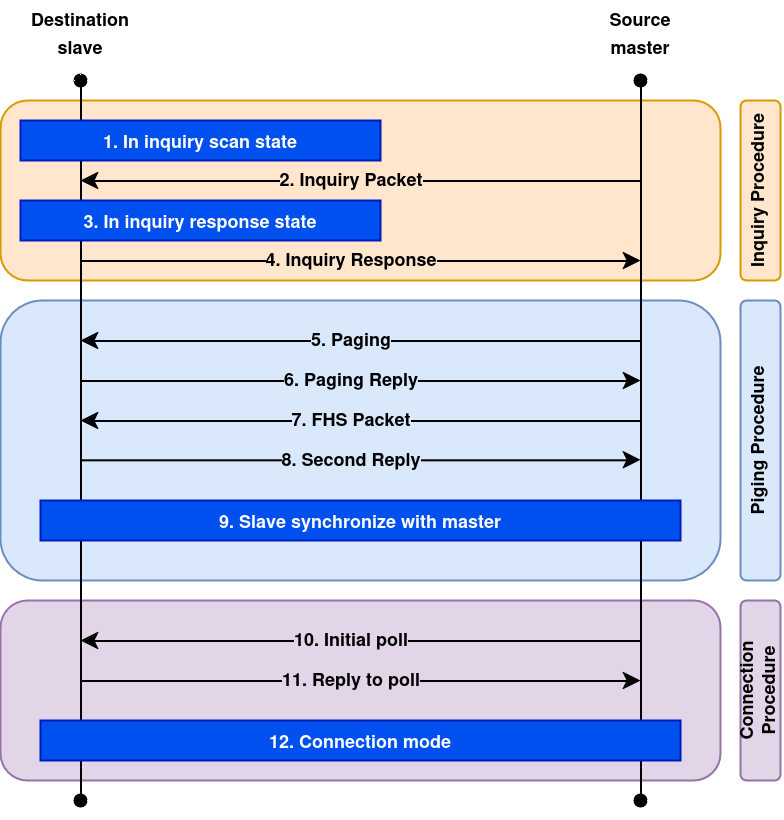
\includegraphics[width=0.75\textwidth]{img/ble_con}
    \caption{Connection Procedure in Bluetooth}
    \label{fig:ble_con}
\end{figure}

Like show in Fig.~\ref{fig:ble_con}:
\begin{itemize}[nosep]
    \item \textbf{\textit{Inquiry Procedure}}: the goal of this part is to retrive the information of each nearby nodes. A node run an inquriy scan and any listening device for this type of request, replies with its address, name and other info.
    \item \textbf{\textit{Paging Procedure}}: the purpose of this process is to create a connection between two bluetooth device. Each device \textbf{must knows} the address of the other. \textbf{\textit{FHS}}: \textbf{Frequency Hopping Sequence}.
    \item \textbf{\textit{Connection Procedure}}: after the \textit{paging} process it is necessary to define the \textbf{connection state}.
\end{itemize}

\subsection{Connection}
A bluetooth connection can have four kinds of mode:
\begin{enumerate}[nosep]
    \item \textbf{\textit{active mode}}: this is regular connected mode, where the device is actively transmitting or receiving data.
    \item \textbf{\textit{sniff mode}}: the device is active periodically for a certain amount of time (\textit{power-saving mode}).
    \item \textbf{\textit{hold mode}}: is a temporary, power-saving mode where a device sleeps for a defined period (not necessarily periodic) and then returns back to active mode when the interval passed. The master can command a slave device to hold.
    \item \textbf{\textit{park mode}}: when the master command a slave to ``park'', that slave become inactive until the master tells it to wake up.
\end{enumerate}

\subsection{Pairing}
\begin{boxA}
    Paired devices automatically establish a connection whenever thery are close enough. No UI interaction are required.
\end{boxA}
When device pair up, they share their address, name and profiles. Usually all this information are stored in memory. They also share common \textbf{secret key}, which allow them to bond whenever they want. \\
Pairing usually requires an \textbf{authentication process} where a user must validate the connection between devices, it could be different depending on the domain, some device ask to \textbf{press a button} (headset) or other can ask to \textbf{insert a code} (PC or smartphone).

\newpage
\subsection{Power Class}
The transmit power and therefore range, of a bluetooth module is defined by its \textbf{power class}. There are three defined class power:
\begin{center}
    \begin{tabular}{ | c | c | c | c | } \hline
        \textbf{Class number} & \textbf{Max Output Power}$_{dBm}$ & \textbf{Max Output Power}$_{mW}$ & \textbf{Max Range} \\ \hline
        \textbf{class 1} & 20 & 100 & 100m \\ \hline
        \textbf{class 2} & 4 & 2.5 & 10m \\ \hline
        \textbf{class 3} & 0 & 1 & 10cm \\ \hline
    \end{tabular}
\end{center}

\subsection{Profiles}
While bluetooth \textbf{specification} define how the technology \textit{works}, \textbf{profiles} define how it is \textit{used}. Two bluetooth device are \textbf{compatible} if they \textbf{support the same profiles}. Some explanation of the most common bluetooth profiles:
\begin{itemize}[nosep]
    
    \item \textbf{\textit{Serial Port Profile}} (\textbf{\textit{SPP}}): permit to substitute a serial communication protocol (like RS-232 or UART). \textit{SPP} is great for sending data between two device

    \item \textbf{\textit{Human Interface Device}} (\textbf{\textit{HID}}): is the profile to enable the receiving data from the user-input device (like mice, keyboard or joystick). \textbf{Bluetooth HID} substitute \textbf{HID} alredy defined for human input USB device, the innovation is the substitution of the USB cable for the communication.

    \item \textbf{\textit{Hands-Free Profile}} (\textbf{\textit{HFP}}) and \textbf{\textit{Headset Profile}} (\textbf{\textit{HSP}}): \textit{HFP} implements a few features on top of \textit{HSP} to allow common phone interaction (accepting/rejecting calls, etc.) that occur while the phone remains in your pocket.

    \item \textbf{\textit{Advanced Audio Distribution Profile}} (\textbf{\textit{A2DP}}): \textit{A2DP} define how audio can be transmitted from one bluetooth device to another. \textit{HFP} and \textit{HSP} have a bidiretion communication, instead \textit{A2DP} is one-way street, that permit higher quality potential.

    \item \textbf{\textit{A/V Remote Control Profile}} (\textbf{\textit{AVRCP}}): the audio/video remote control profile allows for remote controlling of a bluetooth device. It is usually implemented alongside \textit{A2DP} to allow the remote speaker to tell the audio-sending device fast-forward, rewind, etc.

\end{itemize}

\subsection{Bluetooth Stack}

\begin{figure}[h]
    \centering
    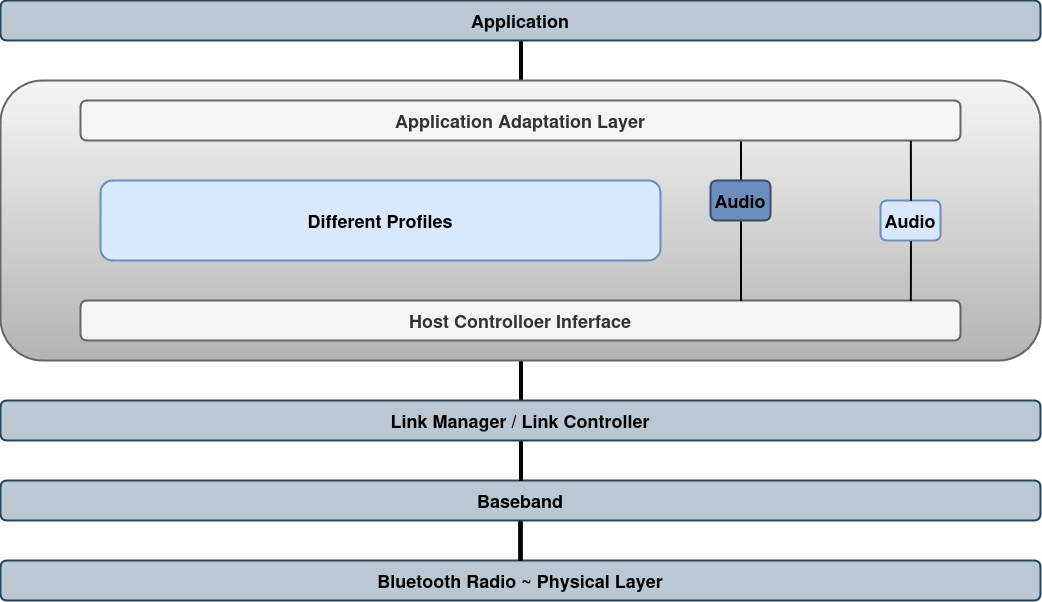
\includegraphics[width=0.85\textwidth]{img/ble_stack}
    \caption{Bluetooth Stack}
    \label{fig:ble_stack}
\end{figure}

The bluetooth protocol stack is split in two parts: a \textbf{controller stack} (in Fig.~\ref{fig:ble_stack} the blu/gray section) containing the timinig critical radio interface and \textbf{host stack} (in Fig.~\ref{fig:ble_stack} the biggest container) dealing with high level data. \\ \newline
\textbf{\textit{Radio Layer}} \\
The bluetooth radio layer is used for transmit bit from master to slave (or vice-versa) and it is similar to \textit{physical layer} in ISO/OSI model. It is a \textbf{low-power system} with 10 meters range operating in the same frequency of WiFi and ZigBee: $2.4GHz$. It defines the specification for the transceiver device:
\begin{enumerate}[nosep]
    \item \textbf{\textit{Frequency Bands and Channel Arrangement}} (\textbf{\textit{FHSS}})
    \item \textbf{Transmitter Characteristics}
    \item \textbf{Receiver Characteristics}
\end{enumerate}
The \textbf{\textit{Frequency Hopping Spread Spectrum}} is used for the transmission. The \textbf{Spectrum Spreading} is obtain by hopping between 79 frequency segments distributed between $2.402GHz$ and $2.480GHz$ ($1MHz$). The transmitter and receiver stay on one of this channels for a certain time and then hop to another channel. This system implement \textbf{Frequency Division Multiplexing} (\textbf{FDM}) and \textbf{Time Division Multiplexing}

\begin{figure}[h]
    \centering
    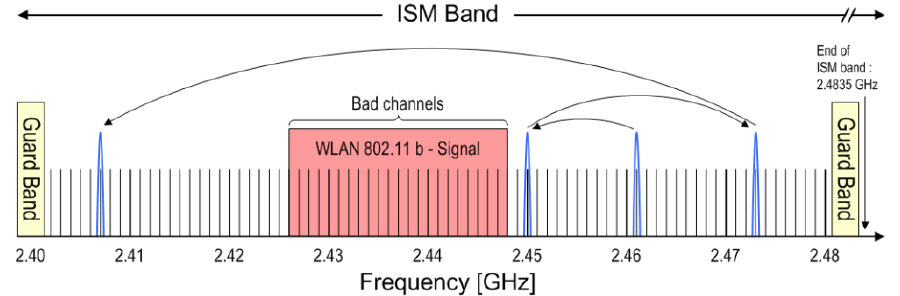
\includegraphics[width=0.75\textwidth]{img/ble_fhss}
    \caption{Frequency Hopping Spread Spectrum}
\end{figure}
The changes of frequency it could be performed in two different way:

\begin{figure}[h]
    \centering
    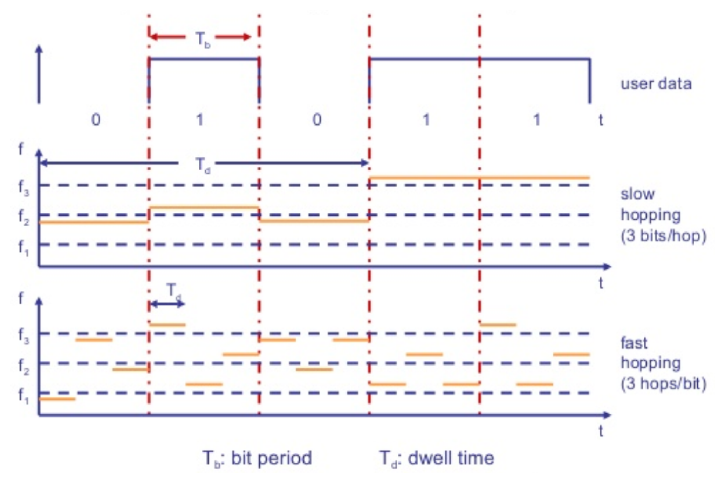
\includegraphics[width=0.75\textwidth]{img/ble_hop}
\end{figure}
\begin{itemize}[nosep]
    
    \item \textbf{\textit{slow hopping}}: the transmitter uses one frequency for several bit period:
    \begin{itemize}[nosep]
        \item typically cheaper (relaxed sync constraints, more time per slot)
        \item not immune to narrowband interferances
    \end{itemize}
    
    \item \textbf{\textit{fast hopping}}: the transmitter uses several frequencies for one period:
    \begin{itemize}[nosep]
        \item typically expensive (hard sync constraints, more slot jumps and high resync frequency)
        \item almost immune to narrowband
        \item rate 1600 hops/sec: $625 \mu s$ of slot time
    \end{itemize}

\end{itemize}
\textbf{\textit{Baseband Layer}} \\
While the \textbf{radio layer} is controlled by the transceiver, the \textbf{baseband layer} is implemented by the controller of a device how want to transmit in bluetooth. The \textit{baseband} is the \textbf{physical layer} of the bluetooth and is used to manages physical channel and links, but also \textit{error connection}, \textit{data whitening}, \textit{hop selection} and \textit{bluetooth security}. \\
Is is used to managed \textbf{synchronous} and \textbf{asynchronous} links. It handles packet and perform the \textit{inquiry} and the \textit{paging} for create connection with nearby device. The baseband layer applies a \textbf{time division duplex} (\textbf{TDD}) scheme to alternating transmitter and receiver. Baseband handles two types of links:
\begin{enumerate}[nosep]
    \item \textbf{\textit{Synchronous Connection Oriented}} link (\textbf{\textit{SCO}}): is a symmectric point-to-point link between a master and a single slave in the piconet. The master maintains the \textit{SCO} link by using reserved slot at regular intervals:
    \begin{itemize}[nosep]
        \item \textit{SCO} is commonly used for the transmission of voice information.
        \item master can support up to three simultaneously \textit{SCO} links, instead, slave only two (sometimes three).
        \item \textit{SCO} packets are never re-transmitted, normally used for $64kB/s$ speech transmission.
    \end{itemize}
    \item \textbf{\textit{Asynchronous Connection Less}} link (\textbf{\textit{ACL}}): is point-to-multipoint between the master and all the slave present in the piconet. In the slot not reserved for the \textit{SCO} links, the master can establish an \textit{ACL} link to any slave
    \begin{itemize}[nosep]
        \item slave alredy into a \textit{SCO} communication are included.
        \item only a single \textit{ACL} link can exist.
        \item for most of \textit{ACL} packets, re-transmission is applied.
    \end{itemize}
\end{enumerate}
These means that \textit{SCO} does not need a connection, there is not an acknoledgement (like \textbf{UDP}), instead the \textit{ACL} need the \textit{ACK} to check if the message needs to be re-transmitted (like \textbf{TCP}). \\
\textbf{\textit{Bluetooth Packet}}
\begin{center}
    \begin{tabular}{ | c | c | c | c | } \hline
        \textbf{bits} & 72 & 54 & 0 - 2745 \\ \hline
        \textbf{description} & \textbf{access code} & \textbf{header} & \textbf{payload} \\ \hline
    \end{tabular}
\end{center}
\begin{enumerate}[nosep]
    \item \textbf{\textit{access code}}: is used for \textit{time synchronization}, \textit{offset compensation}, \textit{paging} and \textit{inquiry}.
    \item \textbf{\textit{header}}: contains information for \textit{packet acknoledgement}, \textit{packet numbering} for out-of-order packet reordering, \textit{flow control}, \textit{slave address} and \textit{error check} for header.
    \item \textbf{\textit{payload}}: can contain either voice field, data field or both. The payload will also contain a \textbf{payload header}.
\end{enumerate}
\textbf{\textit{Other Baseband Function}} \\
The baseband makes other features available like:
\begin{enumerate}[nosep]
    \item \textbf{\textit{error correction}}:
    \begin{itemize}[nosep]
        \item $\frac{1}{3}$ \textbf{rate FEC} (\textbf{Forward Error Correction}): every bit is repeated three times (\textbf{rendundancy}), in this way the receiver can discard up to two bits and validate the transmission.
        \item $\frac{2}{3}$ \textbf{rate FEC}: it use a \textit{polynomial generator} to \textbf{encode} ten bits code into fiftheen bits code.
        \begin{boxA}
            If i want to send $1010001111$ that is ten bits long, i divide into two pieces: $10100$ and $01111$ and i will compute the XOR: $10100 \oplus 01111 = 11011$. I will send the three concatenated values: $m = [10100, 01111, 11011]$. The receiver it could receive wrong the second value, but it can rebuild it performing the XOR between the first and third value. It allow only one ``wrong'' value, if not it can not reconstruct the original message.
        \end{boxA}
        \item \textbf{ARQ scheme} (\textbf{Automatic Repeat Request}): uses \textit{ACK}, \textit{NACK}, \textit{RTO}, etc.
    \end{itemize}
    \item \textbf{\textit{flow control}}: use \textbf{FIFO} queues both in \textit{ACL} and \textit{SCO} links for transmission and receive. In the case that the \textbf{RX FIFO} queues are full, \textbf{flow control} is used to avoid \textbf{congestion} and \textbf{packet drop}. The receiver send a \textbf{stop} indication, the transmitter \textbf{blocks} its \textbf{TX FIFO} queues. When the queues of the receiver are ready it sends an \textbf{go} signal to resume the transmission.
    \item \textbf{\textit{synchronization}}: the piconet is sync using the master clock and it is needed for the transmission at least three information:
    \begin{itemize}[nosep]
        \item \textbf{channel hopping sequence}
        \item \textbf{phase of the sequence}
        \item \textbf{channel access code} to place on the packets (piconet code)
    \end{itemize}
    \item \textbf{\textit{security}}: at link layer, security is maintained by authentication of the peers and encryption of the information. For this basic security we need a public address which is unique for each device, two secret key (authentication keys and encryption keys) and a random number generator.
\end{enumerate}
\textbf{\textit{Link Manager Layer}} \\
On top that layer it is used the \textbf{\textit{Link Manager Protocol}} (\textbf{\textit{LMP}}) that carries out link setup, authentication, link configuration and other protocol. The Link-Controller/Baseband provides services to \textbf{LMP} likes: \textit{authentication}, \textit{pairing}, \textit{encryption}, \textit{change link key}, \textit{slot/clock offset request}, \textit{switch master/slave role}, \textit{hold/sniff/park role} and \textit{quality of service}. \\
\textbf{\textit{Automotive \& Bluetooth}}:
\begin{itemize}[nosep]
    \item \textbf{in-car infortainment system}: permit hands-free audio, calling and application control.
    \item \textbf{remote keyless system}: smart phone are the new key, that use \textit{proximity detection} for locking and unlocking car.
    \item \textbf{in-vehicle wearables}: permit to monitoring the driver health.
    \item \textbf{under-the-hood \& connected maintenance}: allow to transfer diagnostic information.
\end{itemize}
\begin{center}
    \begin{tabular}{ | c | c | c | } \hline
        & \textbf{bluetooth} & \textbf{bluetooth low energy} \\ \hline
        \textbf{freq. band} & $2.4GHz$ ISM Band & $2.4GHz$ ISM Band \\ \hline
        \textbf{no. of channel} & 79, one $1MHz$ & 40, one $2MHz$ \\ \hline
        \textbf{power consumption} & low & less \\ \hline
        \textbf{data rate} & between $1Mbps$ and $3Mbps$ & $1Mbps$ \\ \hline
        \textbf{latency} & $\approxeq$ 100ms & $\approxeq$ 6ms \\ \hline
        \textbf{range} & < 30m & 50m (in open area: 150m) \\ \hline
        \textbf{topology} & peer-to-peer (1:1) & \begin{tabular}{@{}c@{}}peer-to-peer (1:1) \\ star (many:1) \\ broadcast (1:many) \\ mesh (many:many) \end{tabular} \\ \hline
        \textbf{device pairing} & required & not required \\ \hline
        \textbf{voice capable} & yes & no \\ \hline
        \textbf{node/active slave} & 7 & unlimited \\ \hline
        \textbf{security} & 64bits or 128 bits & 128 bits AES \\ \hline
        \textbf{smartphone compatibility} & 100\% & 100\% \\ \hline
        \textbf{use cases} & 
        \begin{tabular}{@{}c@{}}
            streaming application \\ 
            like audio streaming, \\ 
            file transfer and
            \\ headset 
        \end{tabular} & 
        \begin{tabular}{@{}c@{}}
            location beacons, \\ 
            smart home application, \\ 
            medical deivces, \\ 
            industrial monitoring \\ 
            and fitness trackers 
        \end{tabular} \\ \hline
    \end{tabular}
\end{center}

\newpage
\section{LoRa: Long Range}

\begin{figure}[h]
    \centering
    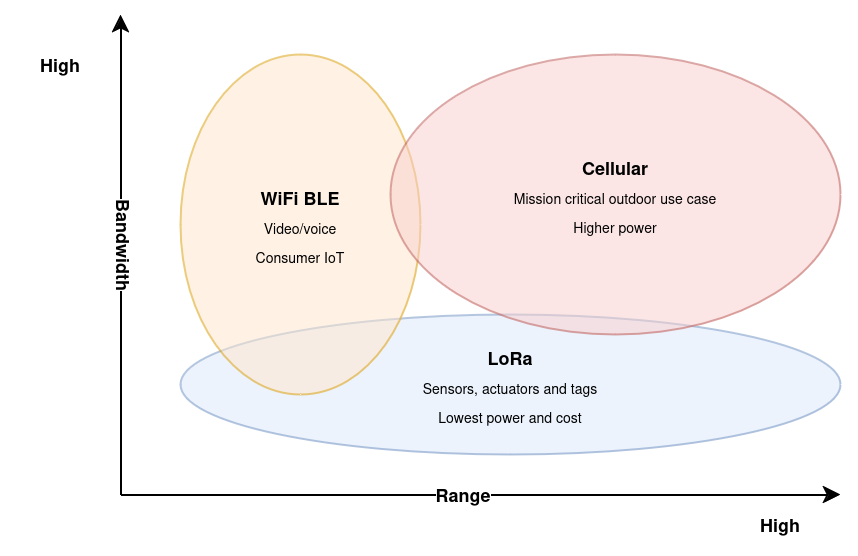
\includegraphics[width=0.5\textwidth]{img/lora}
\end{figure}
\textbf{LoRa} has an unlicenced frequency band equal to: $868MHz$ (in Europe) and very long range coverage: up to \textbf{10 km}. It is composed by two part:
\begin{enumerate}[nosep]
    \item \textbf{LoRa}: the \textit{physical layer} that is \textbf{proprietary}.
    \item \textbf{LoRaWAN}: \textbf{Long Range Wide Area Network} that defines the upper layers (in particular MAC layer).
\end{enumerate}

\newpage
\subsection{LoRa Stack}

\begin{figure}[h]
    \centering
    \begin{minipage}[t]{0.3\textwidth}
        \centering
        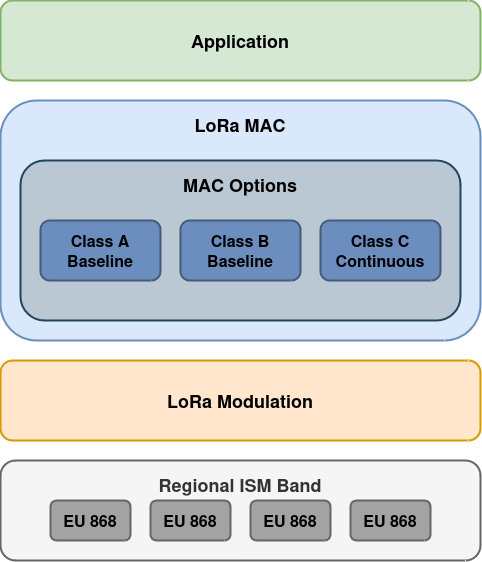
\includegraphics[width=\textwidth]{img/lora_stack}
        \caption{LoRa Stack}
    \end{minipage}
    \begin{minipage}[t]{0.65\textwidth}
        \centering
        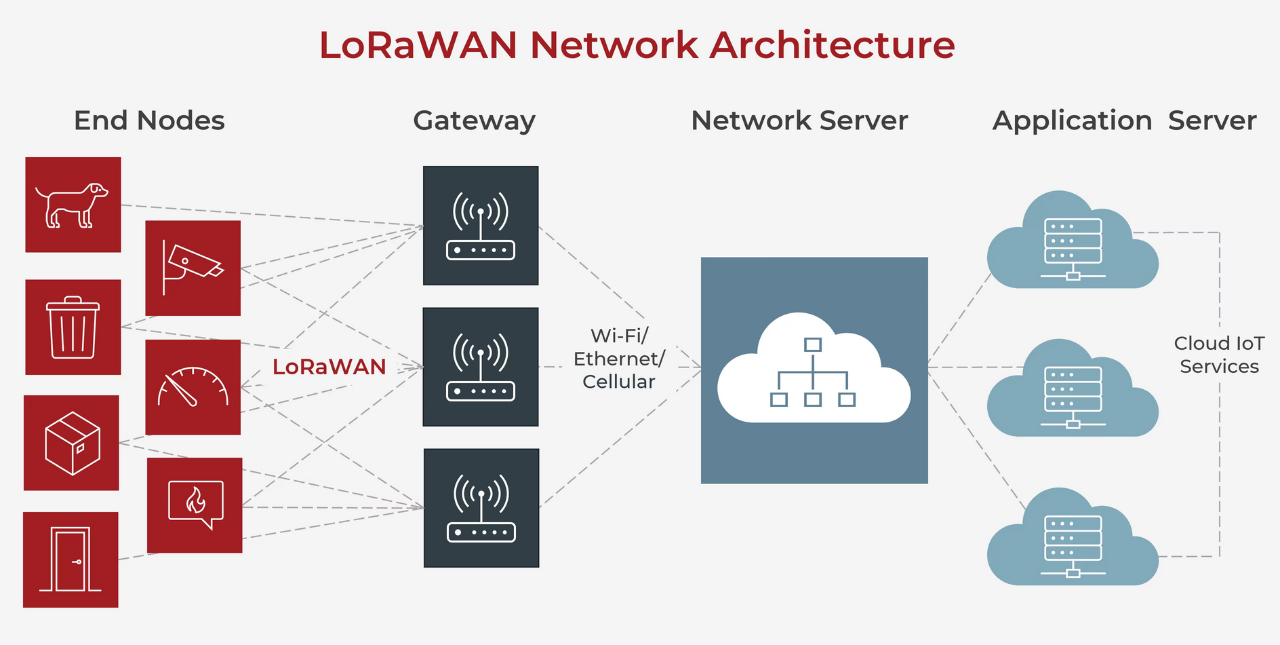
\includegraphics[width=\textwidth]{img/lora_network}
        \caption {LoRaWAN network architecture}
        \label{fig:lora_net}
    \end{minipage}
\end{figure}
\textbf{LoRaWan} defines the \textit{MAC Layer}, the point-to-point network, the communication protocol and the system architecture standard (Fig. \ref{fig:lora_net}). It, also, managed the \textit{frequency}, \textit{data rate} and \textit{power device}.
\begin{itemize}[nosep]
    \item \textbf{end device, node} an embedded object with low-power communication constraints.
    \item \textbf{gateway} receive broadcast data and send data from/to the \textit{end device}.
    \item \textbf{network server} route message from \textit{end device} to the right application, and back.
\end{itemize}
\textbf{\textit{Addressing}}: to each \textit{device} is assign an \textbf{unique identifier} (\textbf{DevEUI}) of 64 bits, instead to each \textit{application} is attribute \textbf{distinctive fingerprint} (\textbf{AppEUI}) of 64 bits, moreover after the access inside a network of a new device it receives a \textbf{dynamic} \textit{non-unique} address of 32 bits (\textbf{DevAddr}). \\ \newline
\textbf{\textit{Frame Counter}} prevent \textbf{replay attack}, to prevent this each nodes (both \textit{end device} and \textit{server}) reject message that contain frame counter that is lower than the expected ones.

\newpage
The \textit{end device} could be classified into \textbf{three different classes}:
\begin{figure}[h]
    \centering
    \begin{minipage}[t]{0.45\textwidth}
        \centering
        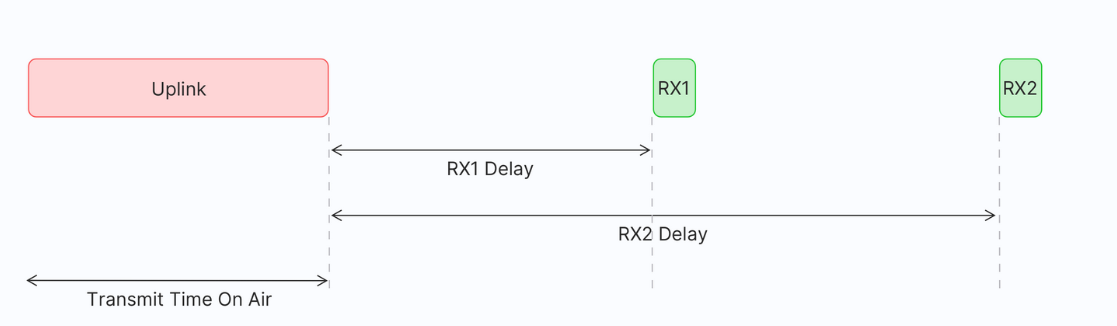
\includegraphics[width=\textwidth]{img/lora_classA}
        \caption{\textbf{Class A}}

        \begin{flushleft}
            Support bidirectional communication (from/to gateway), transmission messages can be sent in any time (random), two possible receive windows at specific time (after 1s and after 2s) after a transmission message, the gateway can reply in one of this two windows.
        \end{flushleft}
    \end{minipage}
    \begin{minipage}[t]{0.45\textwidth}
        \centering
        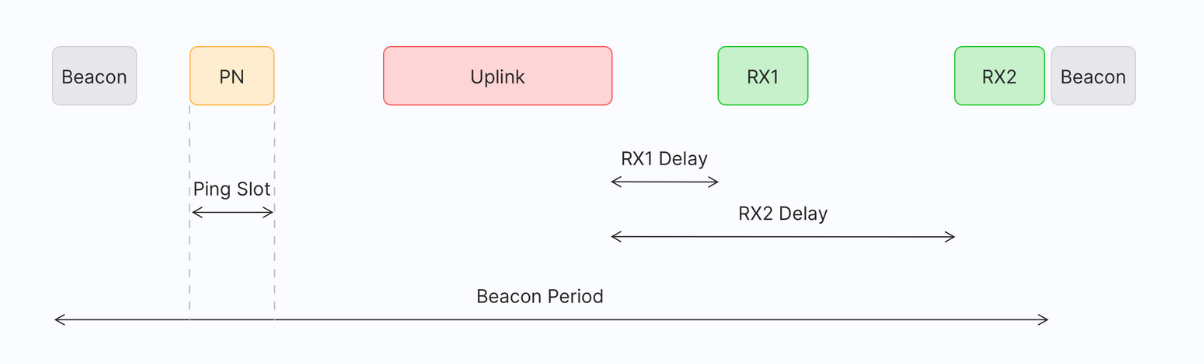
\includegraphics[width=\textwidth]{img/lora_classB}
        \caption{\textbf{Class B}}

        \begin{flushleft}
            Extend \textit{class A} by adding scheduled receive windows for receiving message from the gateway/server. It use time-sync beacons transmitted by the gateway, the \textit{end device} periodically open receive window.
        \end{flushleft}
    \end{minipage}
\end{figure}

\begin{figure}[h]
    \centering
    \begin{minipage}[t]{0.45\textwidth}
        \centering
        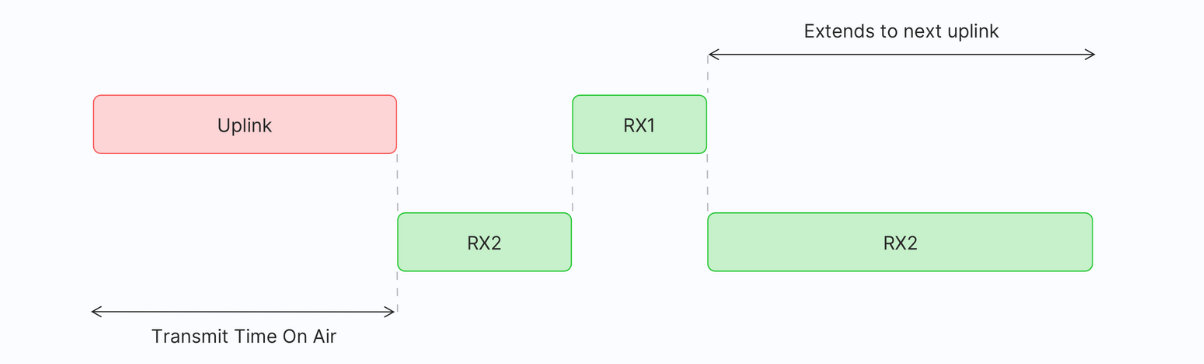
\includegraphics[width=\textwidth]{img/lora_classC}
        \caption{\textbf{Class C}}

        \begin{flushleft}
            Extend \textit{class A} by keeping the receive window open unless they are transmitting. This allow \textbf{low latency} communication, but it consume more energy than \textit{class A} device.
        \end{flushleft}
    \end{minipage}
\end{figure}

\subsection{Secuirty}
LoRaWAN specifies three different class of \textbf{security keys}: \textbf{\textit{NwSKey}}, \textbf{\textit{AppSKey}} and \textbf{\textit{AppKey}}, all have the lenght of 128 bits. The algorithm use for the encryption is \textbf{\textit{AES-128}}. \\
When a device joins the network (called \textbf{activation} or \textbf{join}), an \textit{application session key} (\textbf{AppSKey}) and \textit{network session key} (\textbf{NwSKey}) are generated that will be used for the duration of the session. The \textbf{AppSKey} is the \textit{private key}, instead the \textbf{NwSKey} is the \textit{public key}. The \textbf{Network Session Key} is used for the interaction between the node and the server and it is used to validate the integrity of each message using the \textbf{Message Integrity Code} (\textbf{MIC}). The \textbf{MIC} is similar to checksum expect that it prevents intentional tampering with message (\textbf{AES-CMAC}), it is also used to map the \textbf{DevAddr} to both \textbf{AppEUI} and \textbf{DevEUI}. The \textbf{Application Session Key} is used for encryption and decryption of the payload. \\
The \textbf{Application Key} (\textbf{AppKey}) is only know by the device and the application. The \textbf{NwSKey} and \textbf{AppSKey} are derived from this key. If you dinamically activate the device (\textbf{Over the Air Activation - OTAA}) the two sessione key are regenerate.

\subsection{MAC Commands}
The \textit{end device} and the \textit{server} use \textbf{MAC Commands} for configure the transmission and for the communication.
\begin{itemize}[nosep]
    \item checking connectivity
    \item requesting the status of the device
    \item adapting the data rate of the device
    \item modify channel settings
\end{itemize}

\begin{center}
    \begin{tabular}{ | c | c | } \hline
        \textcolor{green}{\textbf{Pros}} & \textcolor{red}{\textbf{Cons}} \\ \hline
        long range & not realtime data (packet each minutes) \\ \hline
        low power & not use for domotic house (ZigBee or Bluetooth) \\ \hline
        \begin{tabular}{@{}c@{}}
            low cost \\ 
            $\approxeq$ 20\$ per node
        \end{tabular} & watch video (WiFi) \\ \hline
        \begin{tabular}{@{}c@{}}
            low bandwidth \\ 
            between $250bit/s$ and $11kbit/s$
        \end{tabular} & \\ \hline
        \begin{tabular}{@{}c@{}}
            secure: 128 bits \\ 
            end-to-end encryption
        \end{tabular} & \\ \hline
    \end{tabular}
\end{center}

\newpage
\section{V2X}
\textbf{\textit{Intelligent Transportation System}} (\textbf{\textit{ITS}}) add information and communications technology to transport infrastructures and vehicles in effort to improve their safety, relaibility, efficiency and quality $\rightarrow$ avoid congestion (easy work for the drivers). \\ 
\textbf{\textit{European Telecommunication Standard Institute}} (\textbf{\textit{ETSI}}) standardize some new messages that allows to be transmitted into the network: \textbf{\textit{CAM}} and \textbf{\textit{DENM}} to permit safety, a new way to send broadcast message into the network, efficiency and enabling the \textbf{QoS} in the frame. \\

\begin{figure}[h]
    \centering
    \begin{minipage}[t]{0.3\textwidth}
        \centering
        \textbf{\textit{V2X}}
    \end{minipage}
    =
    \begin{minipage}[t]{0.3\textwidth}
        \centering
        \textbf{\textit{IVC}} \\ 
        (\textbf{\textit{Inter-Vehicles Communication}})
    \end{minipage}
    =
    \begin{minipage}[t]{0.3\textwidth}
        \centering
        \textbf{\textit{VANET}} \\ 
        (\textbf{\textit{Vehicle ad-Hoc Network}})
    \end{minipage}
\end{figure}
Different name, but same thing. Today the most used and the standardize one is the \textbf{V2X}, that indicates multiples thigs that can be connect with the vehicle:
\begin{itemize}[nosep]
    \item \textbf{V2V}: vehicular-to-vehicular
    \item \textbf{V2I}: vehicular-to-infrastructure network
    \item \textbf{other}: it depends on top of which domain are created
\end{itemize}
It is possible identify two different \textbf{application} for \textbf{V2X}:

\begin{figure}[h]
    \centering
    \begin{minipage}[t]{0.35\textwidth}
        \centering
        \textbf{\textit{Non Safety Purpose}} \\ ($\cong$ Infotainment): many messages and high data-rate, low latency and low reliability demand.
    \end{minipage}
    \begin{minipage}[t]{0.55\textwidth}
        \centering
        \textbf{\textit{Safety Purpose}} ($\cong$ X-by-Wire): few message (sporadic) and small packet size, high latency and high reliability demand. It is not possible to tollerate false positive or true negative messages.
    \end{minipage}
\end{figure}
Based on the requirements of the domain where we want deploy \textbf{V2X} we can have different application with different characteristics (latency, reliability, area and persistence).

\newpage
\textbf{\textit{Timeline}}

\begin{figure}[h]
    \centering
    \begin{minipage}[t]{0.2\textwidth}
        \centering
        \textbf{\textit{Traditional Network}}
        \begin{itemize}[nosep]
            \item wired
            \item non-moving nodes
            \item static configuration
        \end{itemize}
    \end{minipage}
    $\rightarrow$
    \begin{minipage}[t]{0.35\textwidth}
        \centering
        \textbf{\textit{Mobile ad-Hoc Network}} (\textbf{\textit{MANET}})
        \begin{itemize}[nosep]
            \item wireless
            \item mobile nodes
            \item dynamic configuration
            \item infrastructure (optinal): WiFi and Mobile cellular line.
        \end{itemize}
    \end{minipage}
    $\rightarrow$
    \begin{minipage}[t]{0.35\textwidth}
        \centering
        \textbf{\textit{Vehicular ad-Hoc Network} (\textbf{\textit{VANET}})}
        \begin{itemize}[nosep]
            \item dynamic topologies (could be bus or star)
            \item infrastructure(less)
            \item broadcast or unicast messages
        \end{itemize}
    \end{minipage}
\end{figure}
It is necessary to change the name from \textbf{MANET} to \textbf{VANET} because there is two main different purpose of the network utilization moreover \textbf{VANET} could change its own topologies dynamically.
It is possible to distinguish \textbf{VANET} in two different scenario:
\begin{figure}[h]
    \centering
    \begin{minipage}[t]{0.45\textwidth}
        \centering
        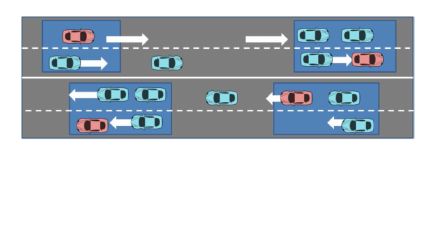
\includegraphics[width=0.75\textwidth]{img/v2x_freeway}

        \begin{flushleft}
            With only ``one direction'' for the movement we can have a \textit{stable connection} (if the vehicles are going in same the way) or \textit{unstable connection}, if the vehicles are not going in the same way (few second of connections).
            \textbf{Autonomous Drive} is drammatic easy on freeway (no cross road or obstacles)
        \end{flushleft}
    \end{minipage}
    \begin{minipage}[t]{0.45\textwidth}
        \centering
        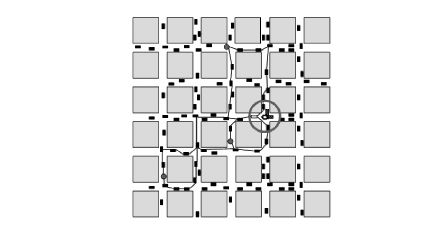
\includegraphics[width=0.75\textwidth]{img/v2x_urban}

        \begin{flushleft}
            There are ``two direction'' for movement. The circumstances can change based on the environment: if the vechicle is driving it can have few neighboard (multiple hops to reach someone faraway), instead in a parking area the number of neighboard it can be easily increase. In the urban scenario it can be possible to have \textit{obstacles}: \textbf{GPS} not always work.
        \end{flushleft}
    \end{minipage}
\end{figure}
\begin{boxA}
    \textbf{\textit{Firmware Over The Air}} (\textbf{\textit{FOTA}}) \\
    \textbf{\textit{Stationary Support Units}} (\textbf{\textit{SSU}}): it is the name give to a nodes that is more important than the other and can have multiple scope:
    \begin{itemize}[nosep]
        \item provide connectivity to other nodes.
        \item manage the radio use for connectivity purpose.
        \item unlimited power supply.
        \item is not connected to internet: is part of the jungle, but more important.
    \end{itemize}
    \textbf{\textit{RoadSide Unit}} (\textbf{\textit{RSU}}): it is an \textbf{SSU} with the internet connection, you can act as a piece of the infrastructure and can enable the traffic to the \textbf{\textit{Traffic Information Center}} (\textbf{\textit{TIC}}).
\end{boxA}
It is possible identify two different \textbf{infrastructure} for \textbf{V2X}:

\begin{figure}[h]
    \centering
    \begin{minipage}[t]{0.45\textwidth}
        \centering
        \textbf{\textit{infrastructure}} \\ (problem alredy solve):
        \begin{itemize}[nosep]
            \item resource management.
            \item add latency (multiple hops).
            \item high load on the \textit{core network}.
            \item high throughput.
        \end{itemize}
    \end{minipage}
    \begin{minipage}[t]{0.45\textwidth}
        \centering
        \textbf{\textit{infrastructureless}}:
        \begin{itemize}[nosep]
            \item self organized: channel access and authentication are the biggest problem.
            \item low latency (no multiple hops).
            \item low datarate: wireless environment in which multiple nodes can communicate simultaneously.
        \end{itemize}
    \end{minipage}
\end{figure}
In the \textbf{infrastructureless} scenario it is necessary to define by your own the rules that the nodes must be compliant to, to allow communication. Moreover there are an heterogeneous scenario to support where the communication can be \textit{point-to-point} or \textit{broadcast}.

\newpage
\begin{figure}[h]
    \noindent
    \begin{minipage}[t]{0.05\textwidth}
        \vfill
        \begin{center} \rotatebox{90}{\textbf{CHALLENGES}} \end{center}
        \vfill
    \end{minipage}
    \begin{minipage}[t]{0.9\textwidth}
        \centering
        \begin{tabular}{
            |p{\dimexpr.35\linewidth-2\tabcolsep-1.3333\arrayrulewidth}
            |p{\dimexpr.55\linewidth-2\tabcolsep-1.3333\arrayrulewidth}|   
        } \hline
        
            \textbf{Communication} & The channel condition dynamically varying based on network topology and the communication type (unicast or broadcast). If multiple nodes want to communicate in the same time it could be happen \textbf{congestion} or \textbf{starvation} on the medium channel \\ \hline

            \textbf{Networking} & The flow information that was send from a node $A$ to a node $B$ can be unicat or multicast (following access algorithm of \textbf{CSMA/CA}). In the same network it can be present multiple different nodes: \textbf{heterogeneity}\\ \hline

            \textbf{Mobility} & Not only for the high speed but for the dynamically change of the topology. It can be predict.\\ \hline

        \end{tabular}
    \end{minipage}
\end{figure}

\section{Wireless Communication}
\begin{enumerate}[nosep]
    \item \textbf{Broadcast Media} (one way): frequency are used for business purposes, you can only receiveing data, like police radio.
    \begin{boxA}
        \centering
        \textbf{\textit{Traffic Message Channel}} (\textbf{\textit{TMC}}) \\
        \textbf{\textit{Radio Distrinbution System}} (\textbf{\textit{RDS}})
    \end{boxA}
    \item \textbf{Cellular Lane}: it is possible to put bottom in \textbf{V2X}. Divide the world into cell (\textbf{\textit{User Equipment - UE}}), each served by base station (\textbf{3GPP} have \textit{license} spectrum frequency).
    \begin{boxA}
        \centering
        \textbf{\textit{Frequency Divide Multiple Access}} (\textbf{\textit{FDMA}}) \\
        \textbf{\textit{Radio Network Core}} (\textbf{\textit{RNC}})
    \end{boxA}
    \item \textbf{IEEE 802.11p}: new communication protocol based on the requirements of the \textbf{V2X}.
\end{enumerate}

\section{C-V2X}
It is the acronym for \textbf{Cellular V2X} and try to embrace the characteristic of \textbf{V2X} on the public system, this type of implementation leads to some problem, like: 
\begin{enumerate}[nosep]
    \item using an infrastructure alredy used for other purpose it is possible to have \textit{delay}.
    \item if the number of the nodes in the infrastructure double (the ones alredy present and all the vehicles plus the RSUs) there are a lot of nodes in the infrastructure. This can lead to \textit{capacity} problems
    \item if we consider that one autonomous car use $4000Gb$ of data per day, it can involve some \textit{bit-rate} problem.
    \item it is \textit{expensive}.
\end{enumerate}
Since the cellular line infrastructure it was create for other purpose, instead the \textbf{V2X}, the downlink and uplink are \textbf{unbalance}, so the communication channel could be:
\begin{enumerate}[nosep]
    \item \textbf{downlink}: from the server to the device the delay is on the order of $10ms$. \textbf{\textit{Forward Access Channel}} (\textbf{\textit{FACH}}).
    \item \textbf{uplink}: from the device to the server, it can have a delay approximately of $50ms$ (if we use \textbf{LTE} it can be lowered until $25ms$). \textbf{\textit{Random Access Channel}} (\textbf{\textit{RACH}}).
    \item there is also a dedicated channel with a delay approximately between $250ms$ and $2s$. \textbf{\textit{Dedicated Transport Channel}} (\textbf{\textit{DCH}}).
\end{enumerate}
It is possible to classified the \textbf{C-V2X} based on the \textbf{radio interfaces} used: \textbf{LTE-Uu} each node is attach to the infrastructure and for communicate each other a node $A$ upload the information on the server and the node $B$ read throught the server (\textit{license spectrum}) or the \textbf{LTE-PC5}, where there is not infrastructure. \\
In the \textbf{LTE-PC5} if you are in the same area of coverage of an antenna you can use the support of the infrastructure (never implemented), instead if you are out of coverage it is possible to use point-to-point commnuication using \textbf{LTE} at $5.9Ghz$ frequency ($\simeq$ 802.11p). \\
The \textbf{physical layer} of \textbf{C-V2X} is divide into \textbf{\textit{Resource Block}} (\textbf{\textit{RB}}) with a width of $180MHz$ each one. Every \textbf{RB} is split into \textbf{\textit{Time Unit}} (\textbf{\textit{TU}}) each one of $1ms$ long. In this way is performed a matrix where on the y-axis there are the \textbf{frequency} and on the x-axis the \textbf{time}. If a node wants to transmit something it needs to take possession of a \textbf{RB} for a certain amount of time ($m$ \textbf{TU}), for each transmission there are two different type of message classes:
\begin{itemize}[nosep]
    \item \textbf{\textit{Transport Block}} (\textbf{\textit{TB}}) where is allocated the data.
    \item \textbf{\textit{Sidelink Control Information}} (\textbf{\textit{SCI}}) that permit to manage the communication: rent a \textbf{RB} for a certain amount of time. In this type of message is included the \textbf{\textit{Modulation and Coding Scheme}} (\textbf{\textit{MCS}}).
\end{itemize}

\begin{figure}[h]
    \centering
    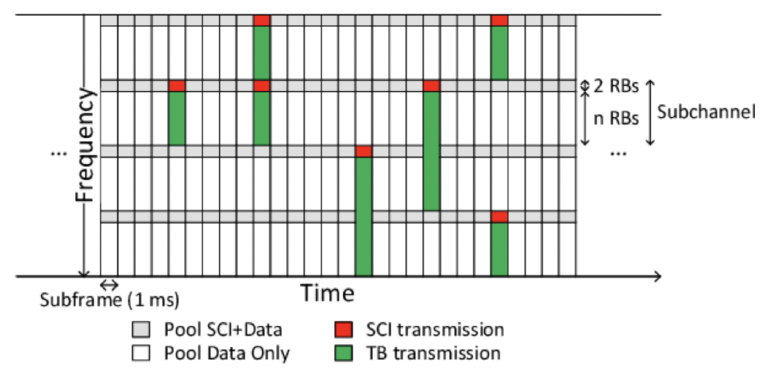
\includegraphics[width=0.75\textwidth]{img/cv2x}
\end{figure}
\textbf{TB} and \textbf{SCI} are transmitted in adjacent \textbf{RBs}, the \textbf{SCI} requires two adjacent \textbf{RB}. The idea behind the medium access is similar to bluetooth, where we change the frequency each time we want to transmit a piece of information, in this case we take a frequency for a certain amount of time for the entire duration of the transmission $\cong$ \textbf{\textit{Time Division Multiple Access}} (\textbf{\textit{TDMA}}) it is mandatory to have synchronize all nodes $\rightarrow$ need \textbf{GPS} and \textbf{GNSS} for the synchronization.

\newpage
\section{802.11p}

\begin{figure}[h]
    \centering
    \begin{minipage}[t]{0.45\textwidth}
        \centering
        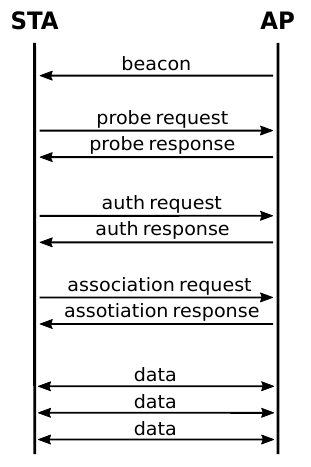
\includegraphics[width=0.45\textwidth]{img/11a}
        \caption{802.11 data flow}
        \label{fig:11a}
        
        \begin{flushleft}
            \textbf{IEEE 802.11} \\
            WiFi: high latency and used by everyone $\rightarrow$ lot of pollution in the world spectrum. It is created for the internet navigation have completly different requirements by \textbf{V2X}. There is no \textbf{QoS} by default. \\
            \textbf{\textit{Basic Service Set}} (\textbf{\textit{BSS}}): there is a node that orchestrate the network (authentication, routing and iP assignement) contain the \textbf{BSSID}. The Fig. \ref{fig:11a} define how a client joining the communication. The server sent a \textbf{beacon} that contain the frequency for that access point and propagate the \textbf{SSID}.
        \end{flushleft}
    \end{minipage}
    \begin{minipage}[t]{0.45\textwidth}
        \centering
        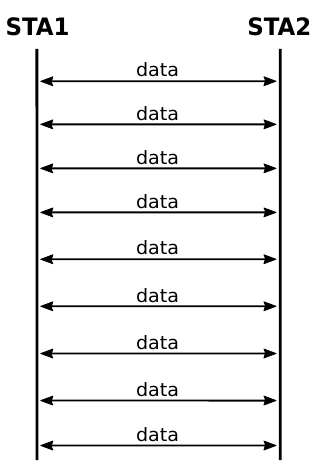
\includegraphics[width=0.45\textwidth]{img/11p}
        \caption{802.11p data flow}
        \label{fig:11p}

        \begin{flushleft}
            \textbf{IEEE 802.11p} \\
            \begin{boxA}
                \centering
                \textbf{bandwidth}: $10MHz$ \\
                \textbf{throughput}: $3-27Mbit/s$ \\
                \textbf{range}: up to $1km$ \\
                \textbf{speed}: $200km/h$
            \end{boxA}
            It is created knowing the requirements for the \textbf{V2X} use the \textit{MAC Layer} of \textbf{802.11a} plus extension:
            \begin{enumerate}[nosep]
                \item random \textbf{MAC address}
                \item use of \textbf{\textit{Enhanced Distributed Channel Access}} (\textbf{\textit{EDCA}}) for prioritizing the message on the medium access (\textbf{QoS})
                \item multi-frequency and multi-radio capabilities
            \end{enumerate}
        \end{flushleft}
    \end{minipage}
\end{figure}
The base idea is of \textbf{802.11p}: there is no need of an iP you can listen and talk on a particular frequency. (Fig. \ref{fig:11p}), is named: \textbf{\textit{Outside The Context of a BSS}} (\textbf{\textit{OCB}}). \textbf{802.11p} is the technologies adopt for the implementation of \textbf{V2X} also known as \textbf{\textit{Wireless Access in Vehicular Environment}} (\textbf{\textit{WAVE}}). Two new tipe of node: \textbf{\textit{RoadSide Unit}} (\textbf{\textit{RSU}}) and \textbf{\textit{On-Board Unit}} (\textbf{\textit{OBU}}).

\subsection{Physical Access}
There are two mainly actor in the \textbf{802.11p} network: the \textit{provider} and the \textit{user}, but there is no technical difference between them. The main task of the \textbf{provider} is to send a \textbf{\textit{On-Deamand Beacon}} ($\simeq$ beacon in \textbf{802.11}) that contain the information and parameter to join the network. The \textbf{physical access} is \textbf{wireless}.

\begin{figure}[h]
    \centering
    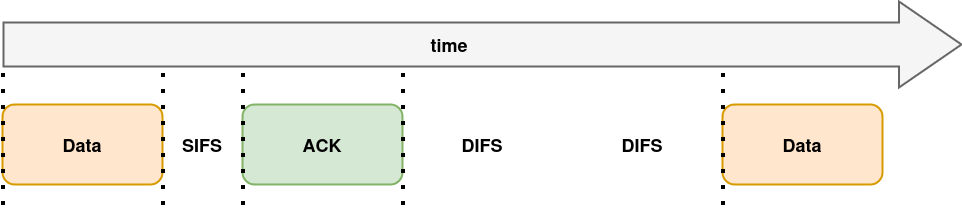
\includegraphics[width=0.55\textwidth]{img/802_11_dcf}
\end{figure}
\begin{boxA}
    \textbf{\textit{Distributed Coordinator Function}} (\textbf{\textit{DCF}}) of \textbf{802.11} two main intervals (it is a time that a station have to wait before transmit):
    \begin{enumerate}[nosep]
        \item \textbf{\textit{SIFS}} - \textbf{\textit{Short Interframe Space}}: before the acknoledgement.
        \item \textbf{\textit{DIFS}} - \textbf{\textit{Data Interframe Space}}: before the data.
    \end{enumerate}
    In a wireless environment it is not possible to anticipate what the other are going to do: \textbf{Carrier Sense} getting a look at the medium listen until is idle, \textbf{Avoid Collision} if the medium is congestionated you can increase the intervals.
\end{boxA}

\subsection{Quality of Service}
Before continue the physical access part on the \textbf{802.11p} small introduction on what is the \textbf{QoS}. Differently from module 1, in this part of course we have \textbf{logical link}, but \textbf{channel/medium wireless}, in this way the priority it cannot be written in the protocol, but must be written in the message and we have to treat according to its rules (written in the msg). \\
$\rightarrow$ give me a packet I will control and I will decided what to do according to the service that you want. \\ \newline
\textbf{QoS} is the overall performance of a telephony or computer network (important for traffic with special requirements $\rightarrow$ different protocols means different requirements). We need to have a \textbf{dedicated QoS} for each \textbf{TCP/iP level}. 
\begin{enumerate}[nosep]
    
    \item \textbf{\textit{H2N}} (include \textit{physical layer} and \textit{data link layer}) 3-bit field called \textbf{\textit{Priority Code Point}} (\textbf{\textit{PCP}}) identify the priority of that frame using these 3-bit:
    \begin{itemize}[nosep]
        \item the type of modulation that we have on the medium $\rightarrow$ \textbf{bitrate}.
        \item bandwidth
    \end{itemize}
    \begin{figure}[h]
        \centering
        \begin{tabular}{ | p{1cm} | p{3cm} | p{7cm} | } \hline
            \textbf{PCP} & \textbf{priority} & \textbf{traffic type} \\ \hline
        \end{tabular} \\
        \begin{tabular}{ | p{1cm} | p{3cm} | p{7cm} | } \hline
            1 & 0 (lowest) & background \\ \hline
            0 & 1 & best effort \\ \hline
            2 & 2 & excellent effort \\ \hline
            3 & 3 & critical application \\ \hline
            4 & 4 & video $<100ms$ latency and jitter \\ \hline
            5 & 5 & voice $<100ms$ latency and jitter \\ \hline
            6 & 6 & internal control \\ \hline
            7 & 7 (highest) & network control \\ \hline
        \end{tabular}
    \end{figure}

    \item \textbf{\textit{Network (iP)}} is used for \textbf{packet schedule} and \textbf{routing protocol}:
    \begin{itemize}[nosep]
        \item \textbf{\textit{IntServ}}: rent a certain resourse for all the router on the path between you and the end node (impossible to actuate except for \textit{bank domain}).
        \item \textbf{\textit{DiffServ}}: every single hop you try to do your best. If there is a packets more important than one other the router try to forward first the most important one. The \textbf{problem} is that this type of control affected the end-to-end performance with all the router performance (the scheduling complexity is not linear).
        \begin{boxA}
            \textbf{\textit{Different Services Code Point}} (\textbf{\textit{DSCP}}) is the method used in networking to classify and manage network traffic by assigning 6.bit value in the iP header, allowing for prioritization of different type of data. $2^6 = 64$ different class. The mainly used are the \textbf{\textit{Per-Hop Behaviour}} (\textbf{\textit{PHB}}):
            \begin{itemize}[nosep]
                \item (default) \textbf{best-effort}
                \item \textbf{\textit{Expedited Forwarding}} (\textbf{\textit{EF}}): low loss and latency traffic.
                \item \textbf{\textit{Assured Forwarding}} (\textbf{\textit{AF}}): assurance of delivery.
                \item \textbf{class selector PHBs}: backword compatibility
            \end{itemize}
        \end{boxA}
        We cannot have a one-to-one conversion from 3-bit of \textbf{H2N} to the 6-bit of \textbf{iP} so it was define a mapping between \textbf{PCP} and \textbf{DSCP}.
        \begin{figure}[h]
            \centering
            \begin{tabular}{ | p{1cm} | p{2cm} | p{2cm} | c | } \hline
                Lv2 & \multicolumn{2}{ | c | }{Lv3} & \multirow{2}{*}{\centering \textbf{Application}} \\ \cline{1-3}
                \textbf{PCP} & \textbf{DSCP} & \textbf{PHB} & \\ \hline
                0 & 0 & 0 & best effort \\ \hline
                1 & 8 & CS1 & torrent \\ \hline
                1 & 10 & AF11 & bulk data \\ \hline
                2 & 16 & CS2 & network management \\ \hline
                2 & 18 & AF21 & transactional data \\ \hline
                3 & 24 & CS3 & call signaling \\ \hline
                3 & 26 & AF31 & mission-critical data \\ \hline
                4 & 32 & CS4 & streaming video \\ \hline
                4 & 34 & AF41 & video conferancing \\ \hline
                5 & 46 & EF & voice \\ \hline
                6 & 48 & CS6 & routing \\ \hline
                7 & 56 & CS7 & network control \\ \hline
            \end{tabular}
        \end{figure}
    \end{itemize}

    \item \textbf{\textit{Transport}}:
    \begin{itemize}[nosep]
        \item \textbf{TCP}: congestion control, fairness among flows and friendliness among TCP algorithm.
        \item \textbf{UDP}: no congestion control, problem delegated at layer three.
    \end{itemize}

    \item \textbf{\textit{Application}}: it became \textbf{Quality of Experience}

\end{enumerate}

\subsection{Physical Access pt.2}
\textbf{802.11} uses \textbf{DCF} for the medium access but for the \textbf{V2X} purpose there are some limitation:
\begin{itemize}[nosep]
    \item there is no congestion control: many station means many collision that produce lower bandwith and have not enough bandwidth means congestive collapse.
    \item no QoS guarantees: there is no difference between packet with higher priority instead of the lower priority.
\end{itemize}
In some cases \textbf{DCF} is replaced by \textbf{\textit{Point Coordination Function}} (\textbf{\textit{PCF}}) but need an infrastructure, that in \textbf{V2X} can be present or not and uses a \textit{centralized function} (present in the \textbf{AP}) for enabling the QoS mechanism. \\ \newline
\textbf{802.11p} uses a \textbf{\textit{Hybrid Coordination Function}} (\textbf{\textit{HCF}}) like policy for the medium access. 
\begin{boxA}
    \textbf{HCF} details:
    \begin{itemize}[nosep]
        \item include the \textbf{802.11e} amendment for the definition of a set of QoS enhancements for wireless LAN application through modification to the media access control layer.
        \item convert the \textbf{DCF} into \textbf{\textit{Enhanced Distributed Channel Access}} (\textbf{\textit{EDCA}}).
        \item convert the \textbf{DIFS} into the \textbf{\textit{Arbitration Interframe Space}} (\textbf{\textit{AIFS}}): it is close to what we have seen in CANBus, permit to associated a number which change according to the priority of the packet that you have to transmit.
        \item defines \textbf{\textit{Traffic Categories}} (\textbf{\textit{TC}}).
    \end{itemize}
\end{boxA}
The core idea is force an application to use an \textbf{AIFS} shorter or larger according to is priority: modify the \textbf{CSMA/CA} using shorter \textbf{AIFS} for higher priority packets.
\begin{boxA}
    \textbf{\textit{Enhanced Distributed Channel Accass}} (\textbf{\textit{EDCA}}) \\
    It is a \textbf{\textit{TCMA}} protocol (\textbf{\textit{Tiered Contention Multiple Access}}) that define the \textbf{AIFS}. It classify user data in four \textbf{Access Categories} (\textbf{AC}): from \textbf{AC0} (lowest priority) to the \textbf{AC3} (highest priority). \\
    It permit to enable \textbf{Burst Mode} using the \textbf{\textbf{Transmission Opportunity}} (\textbf{\textit{TXOP}}): is a bounded time interval during which a station can send many frames as possible, during this period the station does not need to use standard \textbf{EDCA} to access the channel. \\
    Each \textbf{ACs} has different \textbf{\textit{Contention Window}} (\textbf{\textit{CW}}), \textbf{AIFS} and \textbf{TXOP}.
\end{boxA}
In \textbf{802.11p} te four access categories have its own queue and each of then compete in an indipendent way (Fig.~\ref{fig:edca}) to access to the medium (with its own algorithm), instead of \textbf{802.11} we have the \textit{scheduler}, but in the \textbf{11p} is not enough because a device $A$ have to transmit a new packet with higher priority than a packet that the device $b$ have to transmit it can collide with the last one. In this protocol the \textbf{access} is more important tha the \textbf{backbone}.

\begin{figure}[h]
    \centering
    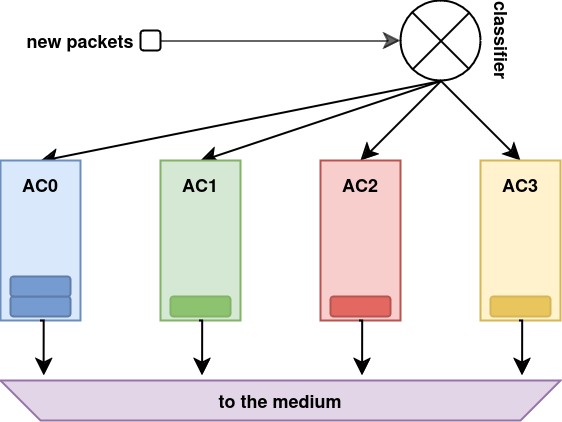
\includegraphics[width=0.45\textwidth]{img/edca}
    \caption{Medium Access - EDCA}
    \label{fig:edca}
\end{figure}
\textbf{HCF} maps eight user priorities with four access categories $\rightarrow$ mapping:

\begin{figure}[h]
    \centering
    \begin{tabular}{ | c | c | c | c | c | c | } \hline
        & \multicolumn{3}{ | c | }{\textbf{802.11p}} & \multicolumn{2}{ | c | }{\textbf{802.11p QoS}} \\ \hline
        priority & \textbf{PCP} & \textbf{Acronym} & \textbf{Traffic Type} & \textbf{AC} &  \textbf{Disignation} \\ \hline
        lowest & 1 & BK & background & AC\_BK & background \\ \hline
        & 2 & - & spare & AC\_BK & background \\ \hline
        & 0 & BE & best effort & AC\_BE & best effort \\ \hline
        & 3 & EE & excellent effort & AC\_BE & best effort \\ \hline
        & 4 & CL & controlled load & AC\_VI & video \\ \hline
        & 5 & VI & video & AC\_VI & video \\ \hline
        & 6 & VO & voice & AC\_VO & voice \\ \hline
        highest & 7 & NC & network control & AC\_VO & voice \\ \hline
    \end{tabular}
\end{figure}

\newpage
Another important table is the definition of the \textbf{EDCA} parameter for the \textbf{802.11p} communication for every type of \textbf{AC}

\begin{figure}[h]
    \centering
    \begin{tabular}{ | c | c | c | c | c | } \hline
        \textbf{AC} & \textbf{CW}$_{min}$ & \textbf{CW}$_{max}$ & \textbf{AIFS} & \textbf{Max TXOP} \\ \hline
        AC\_BK & 15 & 1023 & 9 & 0 \\ \hline
        AC\_BE & 15 & 1023 & 6 & 0 \\ \hline
        AC\_VI & 7 & 15 & 3 & 3.008ms \\ \hline
        AC\_VO & 3 & 7 & 2 & 1.504ms \\ \hline
        legacy DCF & 15 & 1023 & 2 & 0 \\ \hline
    \end{tabular}
\end{figure}

\subsection{802.11p Upper Layer}

\begin{figure}[h]
    \centering
    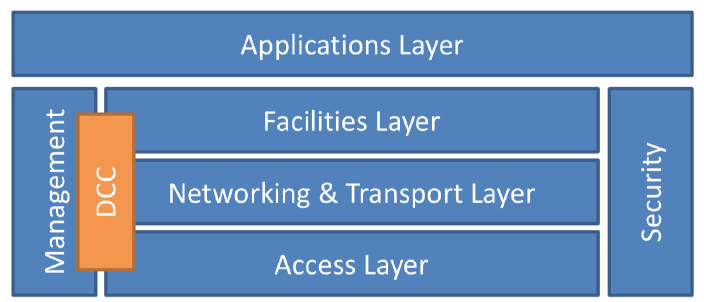
\includegraphics[width=0.75\textwidth]{img/etsi_11p}
    \caption{European Standard for 802.11p}
    \label{fig:etsi_11p}
\end{figure}
\textbf{\textit{Decentralize Congestion Control}} (\textbf{\textit{DCC}}): the environment change based on where we are and so accordin with the environment and the application there are multiple parameter to continuosly read for avoid congestion. It is used an \textbf{\textit{Finite State Machine}} (\textbf{\textit{FSS}}) to know how to set the \textbf{802.11p} parameter for the transmission.
There are three different state:
\begin{enumerate}[nosep]
    \item \textbf{relaxed}: low data rate and high range
    \item \textbf{active}: neutral
    \item \textbf{restrictive}: high data rate and low range
\end{enumerate}
To relax the state (from restrictive to relaxed) the same \textit{maxChannelLoad} must be in the correct range at least for five seconds, instead to limit the state (from relaxed to restrictive) the same \textit{minChannelLoad} must be in the correct range at least for one second, this difference between the transiction direction is to avoid the \textbf{isteresis} that means jumping from a state to another continuosly, polluting the transmission.

\begin{figure}[h]
    \centering
    \begin{minipage}[t]{0.45\textwidth}
        \centering
        \textbf{Input}: will allow us to understand uf we have to change the state, normally is based on the \textbf{channel load} or the \textbf{measured received power} (\textbf{RSS}).
    \end{minipage}
    \begin{minipage}[t]{0.45\textwidth}
        \centering
        \textbf{Output}: each output have an associated value for each state:
        \begin{itemize}[nosep]
            \item \textbf{Transmission Power}: is the bulk movement of electrical energy from a generating site
            \item \textbf{Minimum Packet Interval}: how fast modulate
            \item \textbf{BitRate}: how dealing the contention
        \end{itemize}
    \end{minipage}
\end{figure}

\subsection{ETSI Message}


% PAGINA VUOTA
%\clearpage\null\thispagestyle{empty}\clearpage
%\appendix
%\appendixpage
%\addappheadtotoc

%\clearpage\null\thispagestyle{empty}\clearpage


%\listoffigures


\begin{flushleft}
\bibliographystyle{plain}
\bibliography{sections/references} 
\end{flushleft}

\end{document}
